\chapter[Resultados Experimentais]{Resultados Experimentais}

Este Capítulo visa apresentar os resultados dos testes realizados para avaliar o desempenho do algoritmo proposto na Seção \ref{algPropos}. Foi realizada uma bateria de testes com sequências de vídeos reais, codificadas em JPEG e H.264/AVC. 

Todos os testes foram realizados utilizando os \textit{scripts} do transmissor e do receptor, escritos em \textit{Python} e \textit{Octave} respectivamente, com exceção do processo de estimação de movimento, que se encontra em um arquivo \textit{mex} (linguagem C padrão ANSI), pois trata-se de um processo complexo.

As sequências de vídeo utilizadas foram \textit{akiyo}, \textit{foreman}, \textit{bowing}, \textit{carphone}, \textit{crew}, \textit{flower}, \textit{footbal} e  \textit{mobile}, visualmente apresentadas pela Figura \ref{fig:seg} (ilustradas pelo segundo quadro de cada sequência). Com o propósito de validar o método, tais sequências foram escolhidas por possuírem diversos graus de quantidade de movimento, elementos novos/recorrentes em cena e quantidade/intensidade de alta-frequência impondo assim diversos níveis de dificuldade à super-resolução proposta \cite{silva2009super}.

\begin{figure}[H]
    \centering
    \subfloat[]{
	    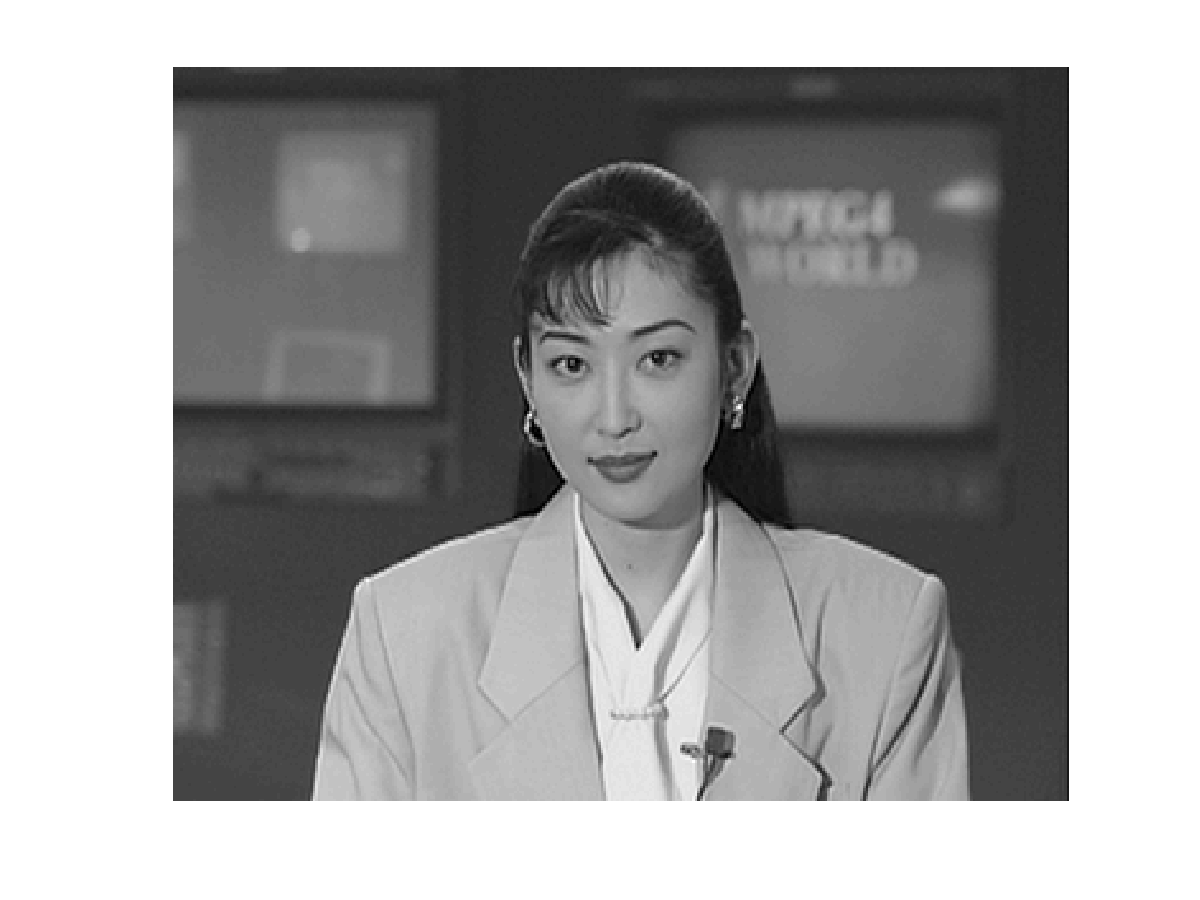
\includegraphics[width=0.4\linewidth]{figuras/akiyo.png}
    }
    \qquad
    \subfloat[]{
    	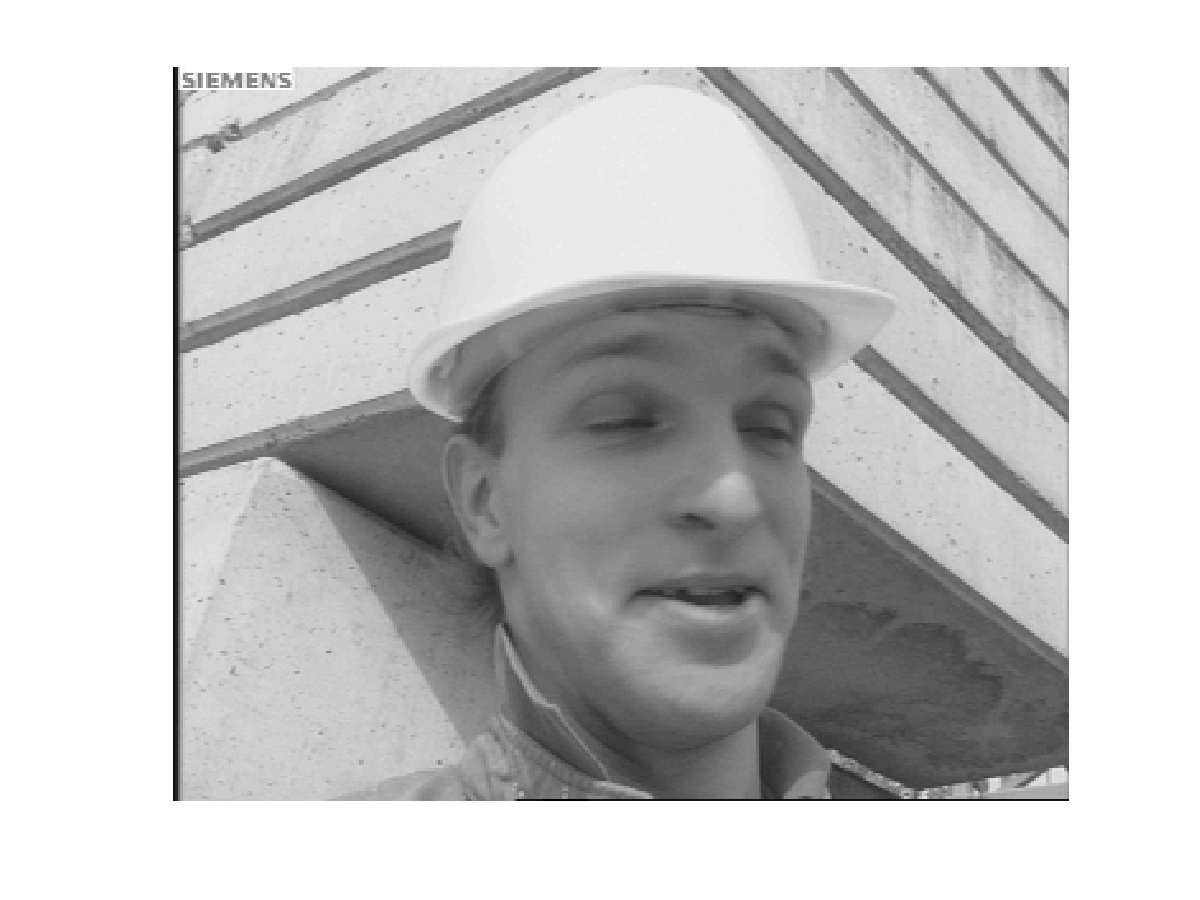
\includegraphics[width=0.4\linewidth]{figuras/foreman.png}
    }
	\qquad
    \subfloat[]{
    	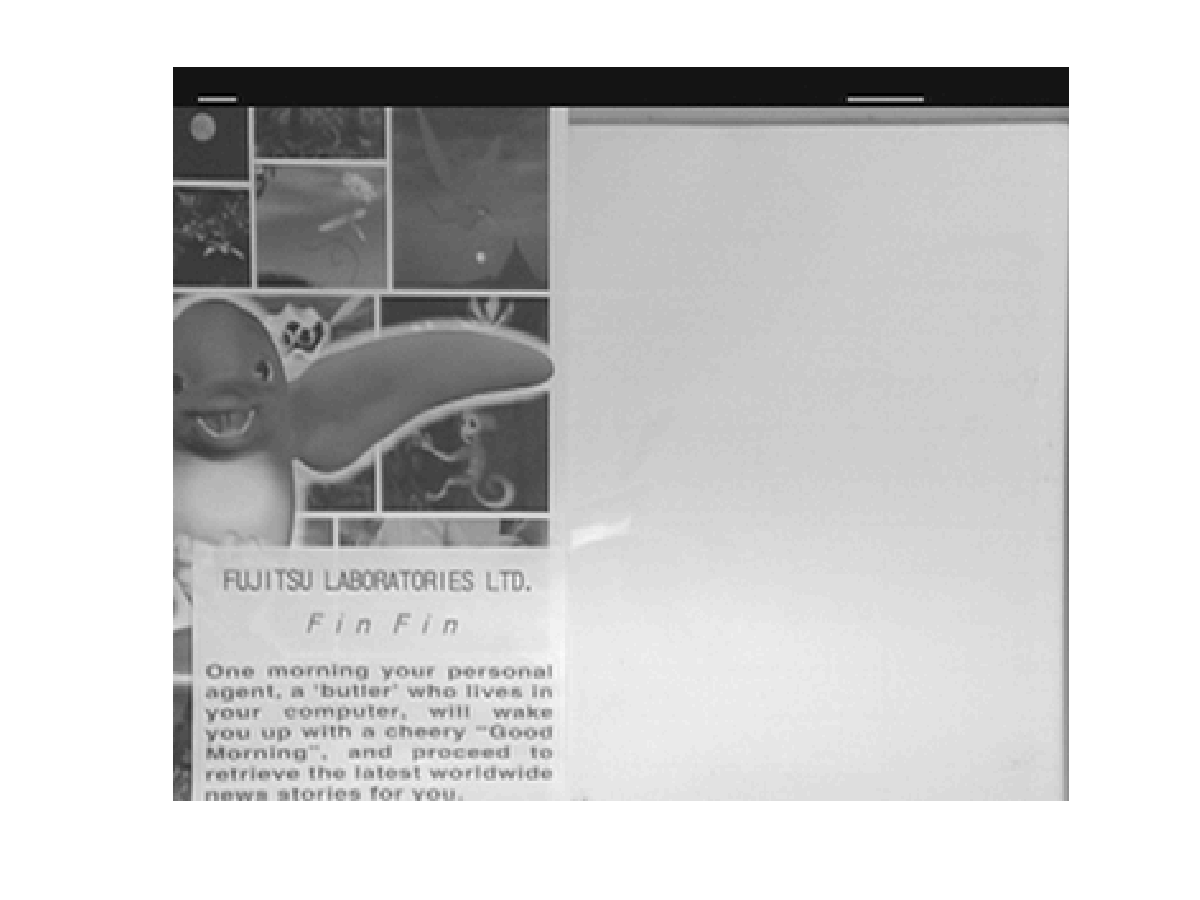
\includegraphics[width=0.4\linewidth]{figuras/bowing.png}
    }
	\qquad
    \subfloat[]{
	    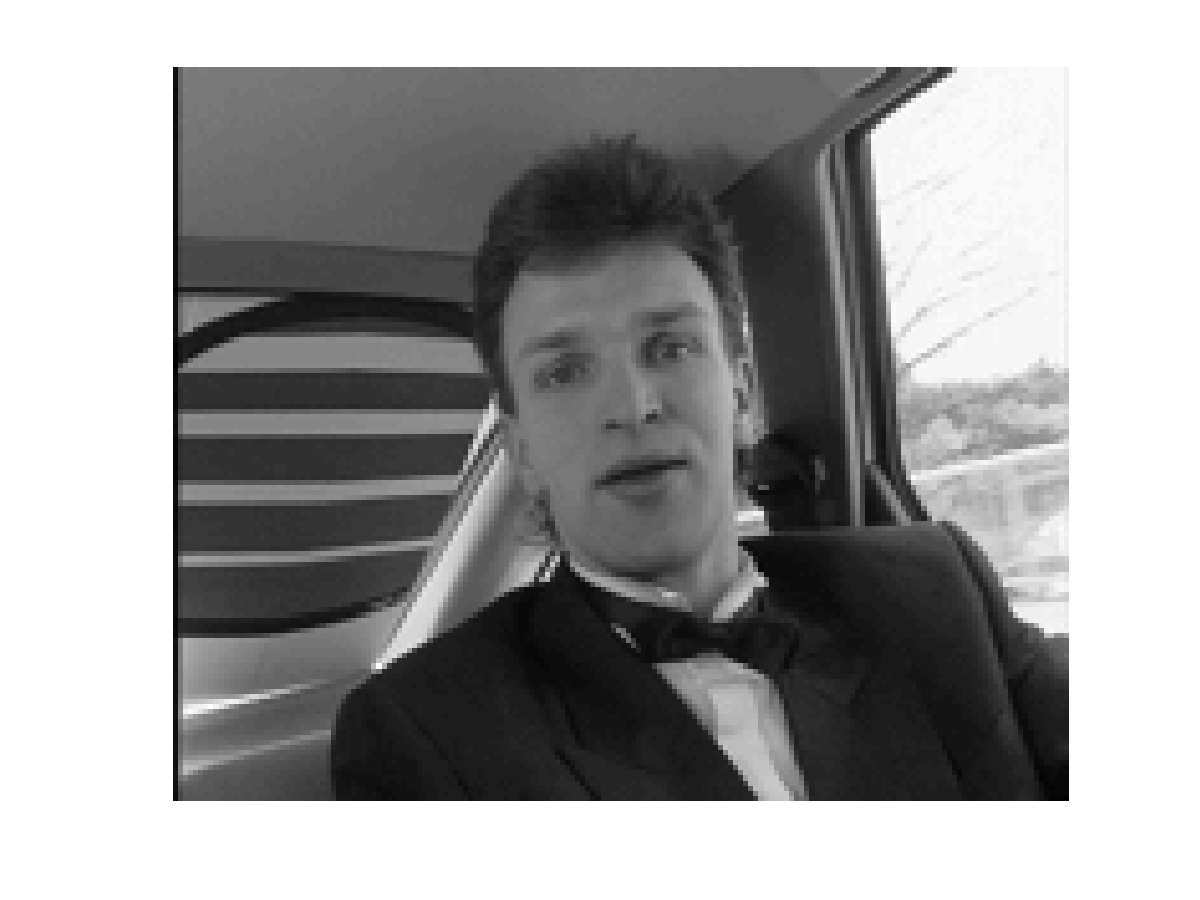
\includegraphics[width=0.4\linewidth]{figuras/carphone.png}
    }
    \qquad
    \subfloat[]{
    	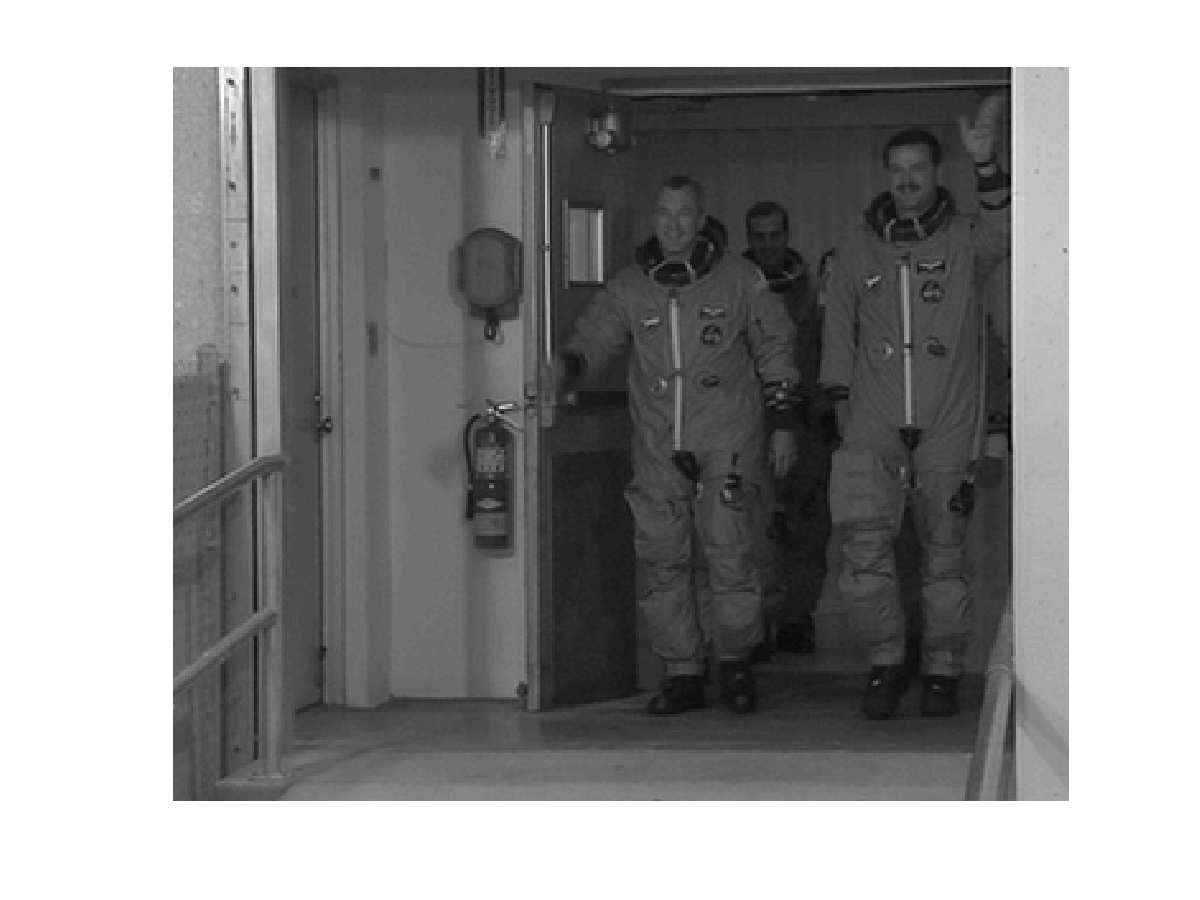
\includegraphics[width=0.4\linewidth]{figuras/crew.png}
    }
	\qquad
    \subfloat[]{
    	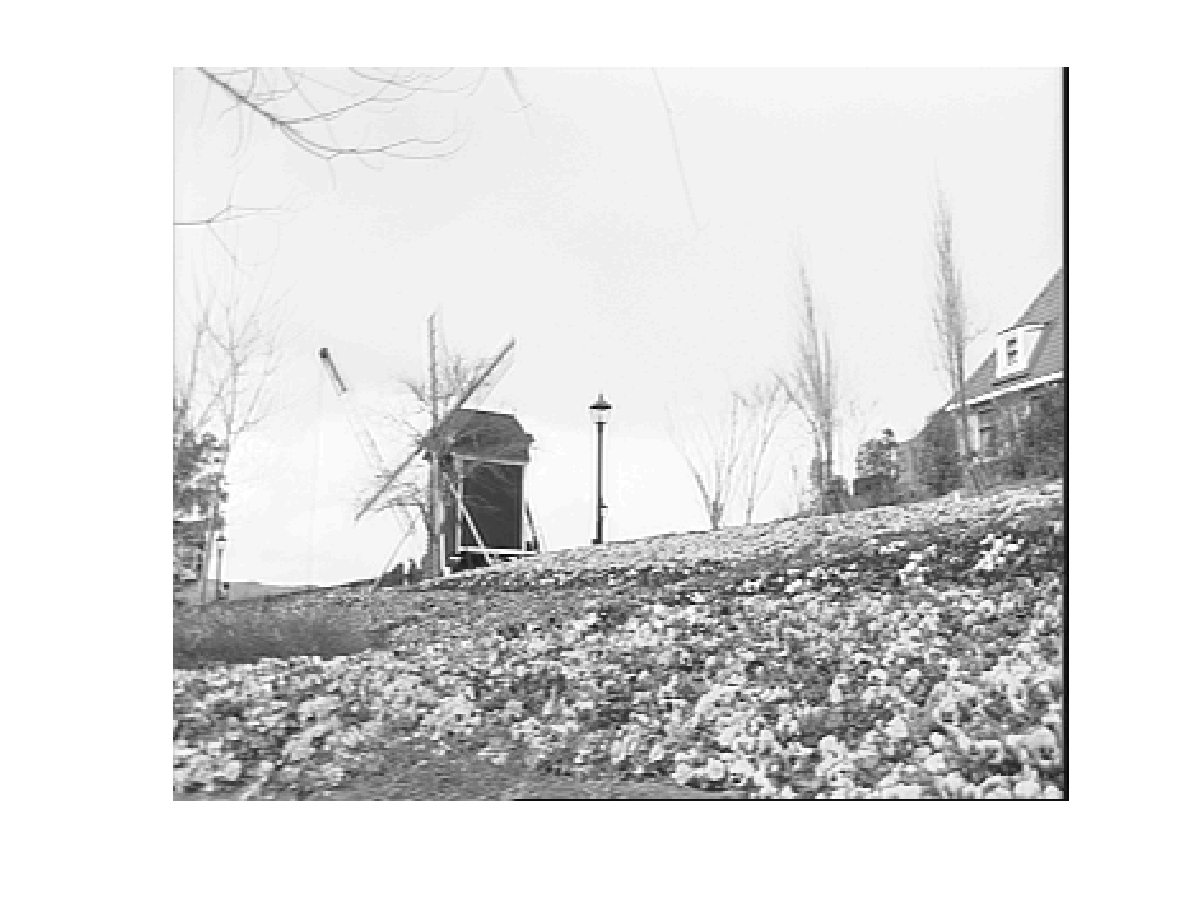
\includegraphics[width=0.4\linewidth]{figuras/flower.png}
    }
	\qquad
    \subfloat[]{
	    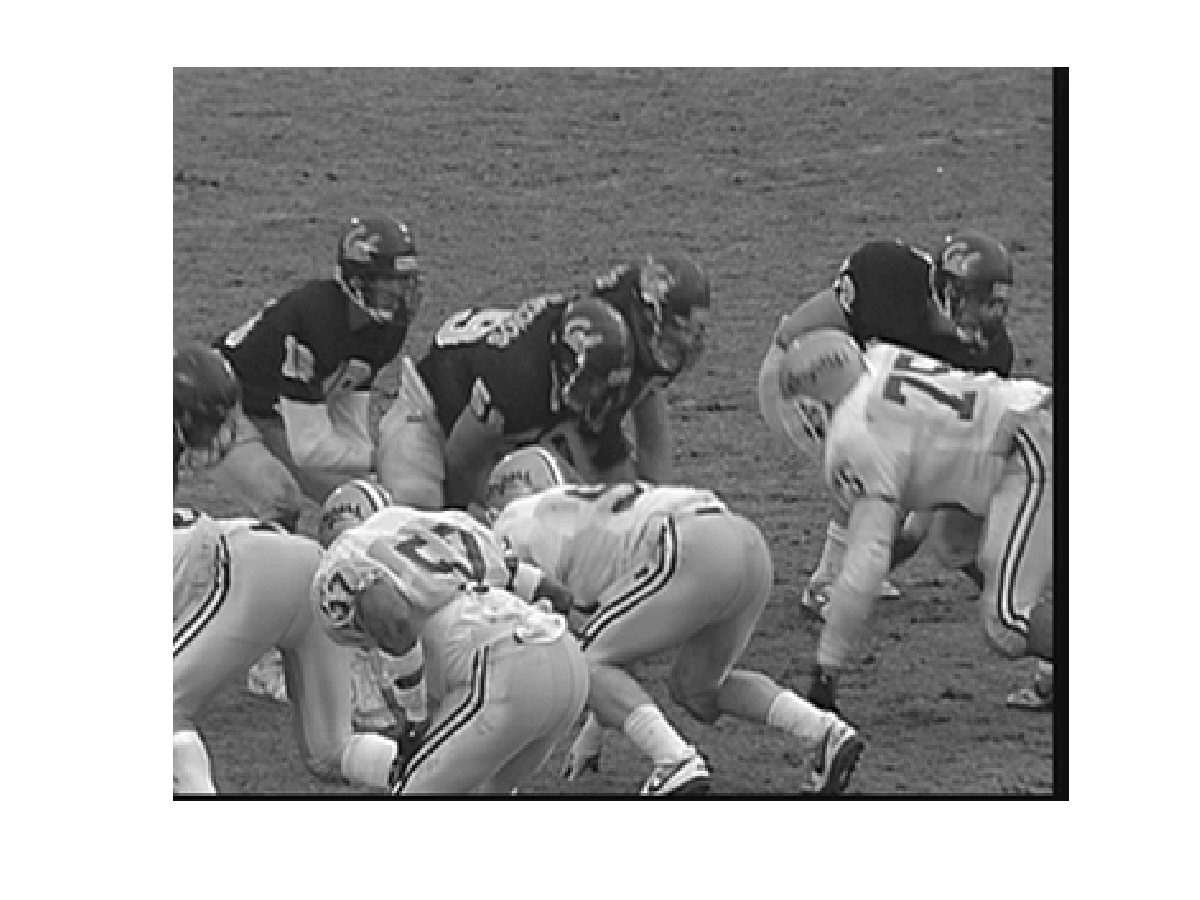
\includegraphics[width=0.4\linewidth]{figuras/football.png}
    }
    \qquad
    \subfloat[]{
    	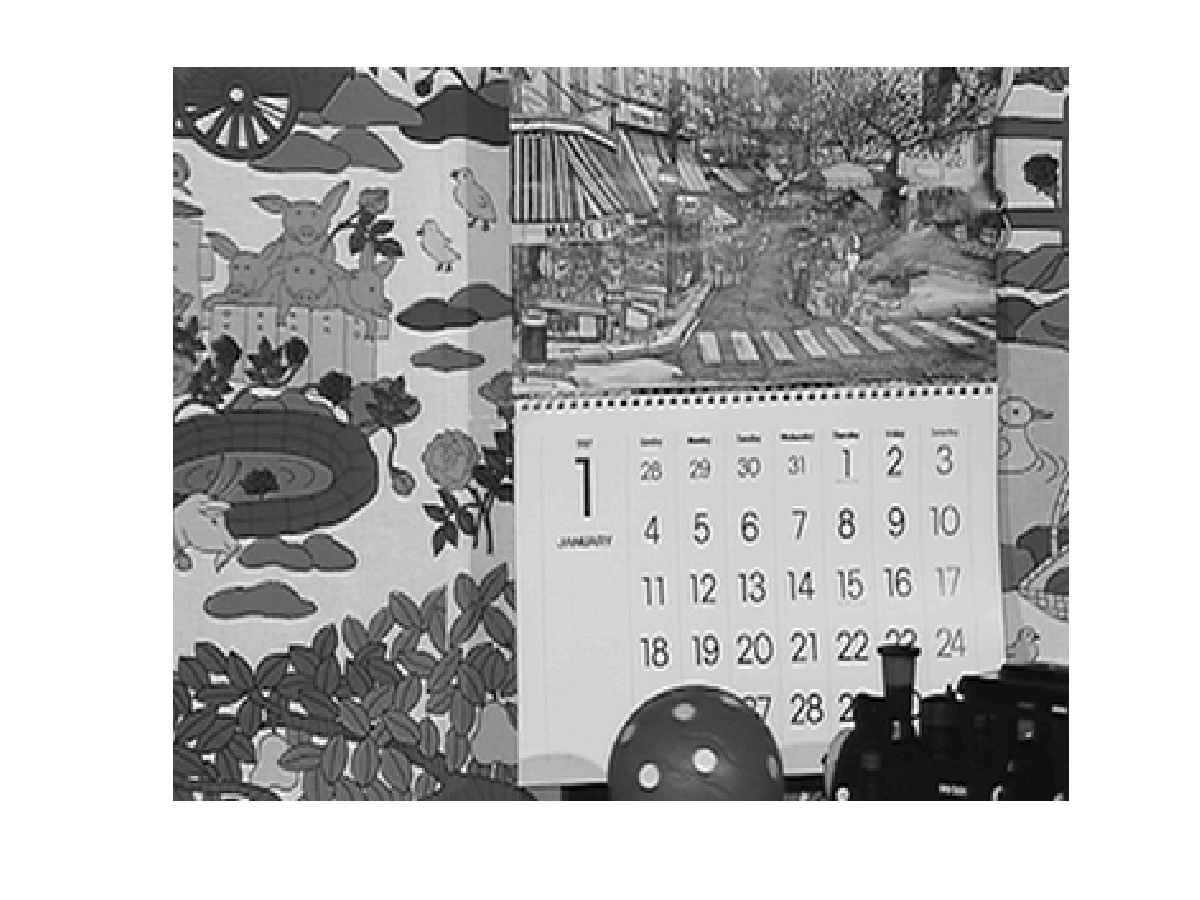
\includegraphics[width=0.4\linewidth]{figuras/mobile.png}
    }

    \caption{Sequências de vídeo : (a)\textit{akiyo}, (b)\textit{foreman}, (c)\textit{bowing}, (d)\textit{carphone}, (e)\textit{crew}, (f)\textit{flower}, (g)\textit{footbal} e  (h)\textit{mobile}.}
	    
    \label{fig:seg}
\end{figure}


\section{Resultados Objetivos}
Nesta Seção serão apresentados resultados objetivos, em formato de gráficos e tabelas, obtidos através de métricas definidas na Seção \ref{metricas}.


\subsection{Teste com codificação JPEG}
A fim de avaliar o desempenho do algoritmo proposto para a decodificação em uma situação prática, aplicou-se ao algoritmo sequências de vídeo codificadas dentre as seguintes condições:
\begin{itemize}
\item Cada sequência foi codificada separadamente utilizando o padrão JPEG, em resolução mista.
\item Aplicou-se valores 2 a 31 ao parâmetro  \textit{qscale}, que é a faixa permitida pelo \textit{software} utilizado para implementação do padrão, o que possibilitou o levantamento das curvas ilustradas nas Figuras \ref{fig:football} e \ref{fig:akiyo}.
\item Utilizou-se o \textit{framework ffmpeg}, especialmente a biblioteca \textit{mjpeg}
para implementar a codificação no padrão JPEG.
\item A luminância foi escolhida para os testes, definindo os quadros originais como referência mediu-se o PSNR médio entre eles e os quadros interpolados, os quadros super-resolvidos e os quadros originais codificados e decodificados.
\item A taxa considerada foi as dos quadros em baixa resolução.
\item Foram utilizados macroblocos de tamanho 8x8 \textit{pixels} e uma janela de busca de 80x80 \textit{pixels} para o processo de estimação/compensação de movimento e para a combinação de altas frequências, e fatores de decimação $M=2$ e $M=4$.
\item Foram medidos os ganhos médios \cite{bjontegaard2001calcuation} de qualidade (PSNR) para o algoritmo proposto em relação aos quadros interpolados. Estes resultados são ilustrados nas Tabelas \ref{GanhoJpeg2} e \ref{GanhoJpeg4}.

\end{itemize}

\begin{figure}[H]
	
	\centering
    \subfloat[]{
		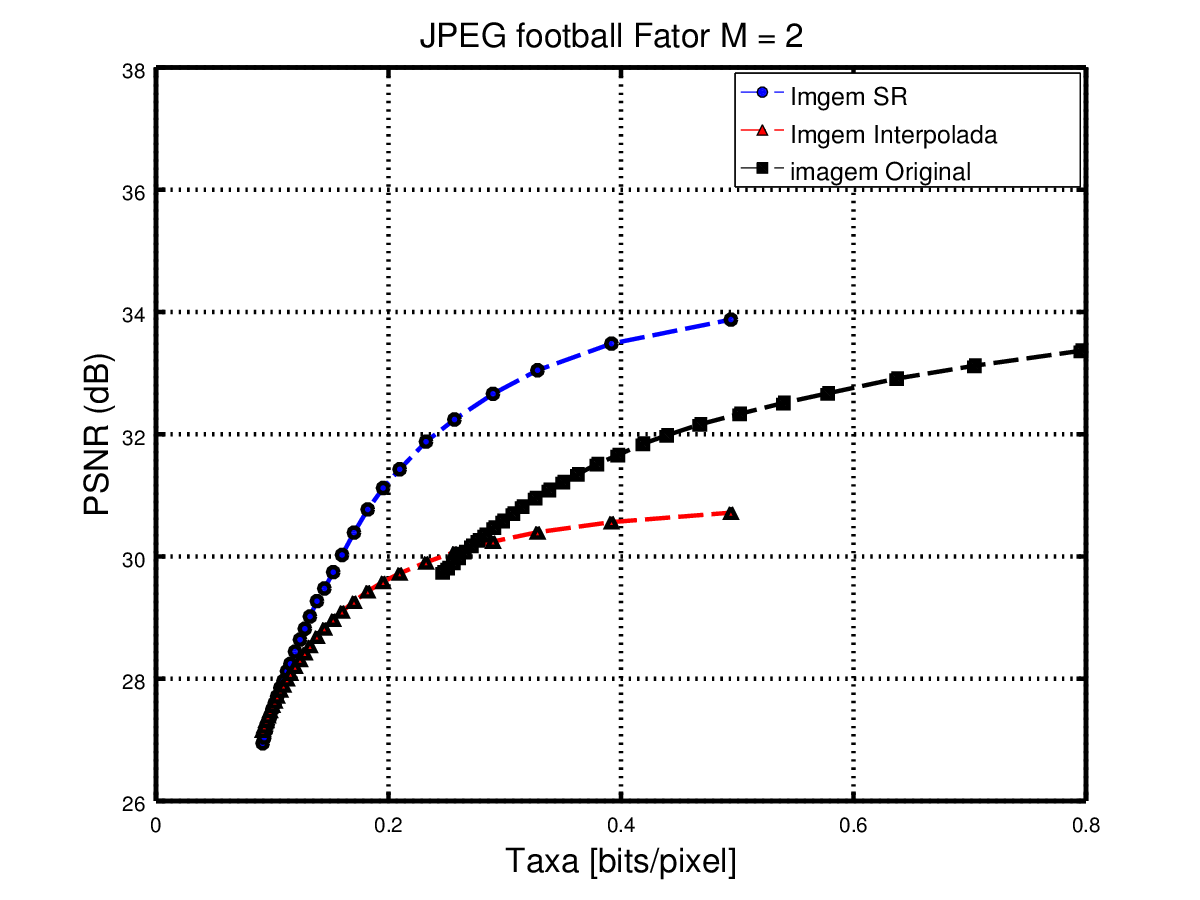
\includegraphics[scale=0.4]{figuras/JPEG_football_Downsampling_factor_2.png}
    }
    \subfloat[]{
	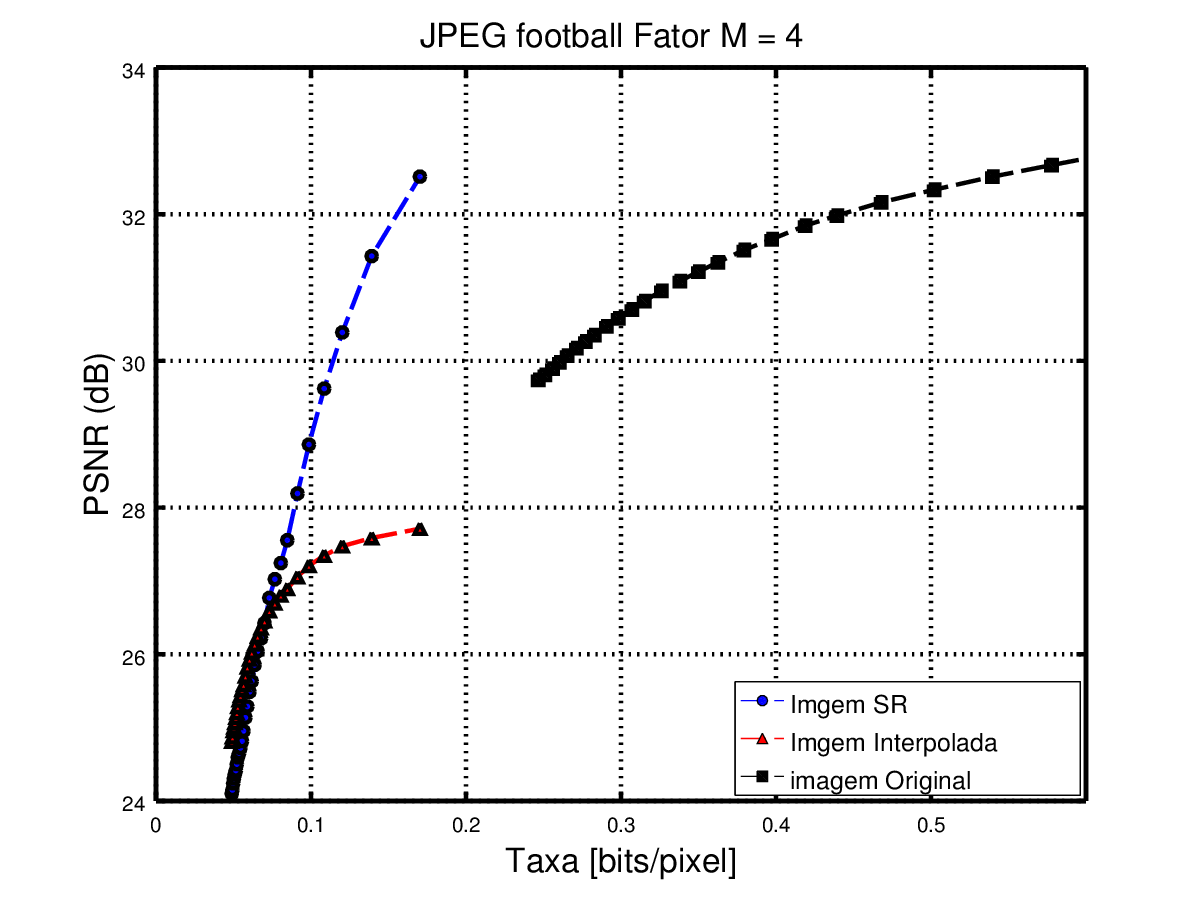
\includegraphics[scale=0.4]{figuras/JPEG_football_Downsampling_factor_4.png}
    }
	\caption{Curva PSNR médio x Taxa, para a sequência de vídeo \textit{Football}: (a) com um fator de decimação $M$ = 2, (b) com um fator de decimação $M$ = 4.}
	\label{fig:football}
\end{figure}


\begin{figure}[H]
	\centering
	\subfloat[]{
		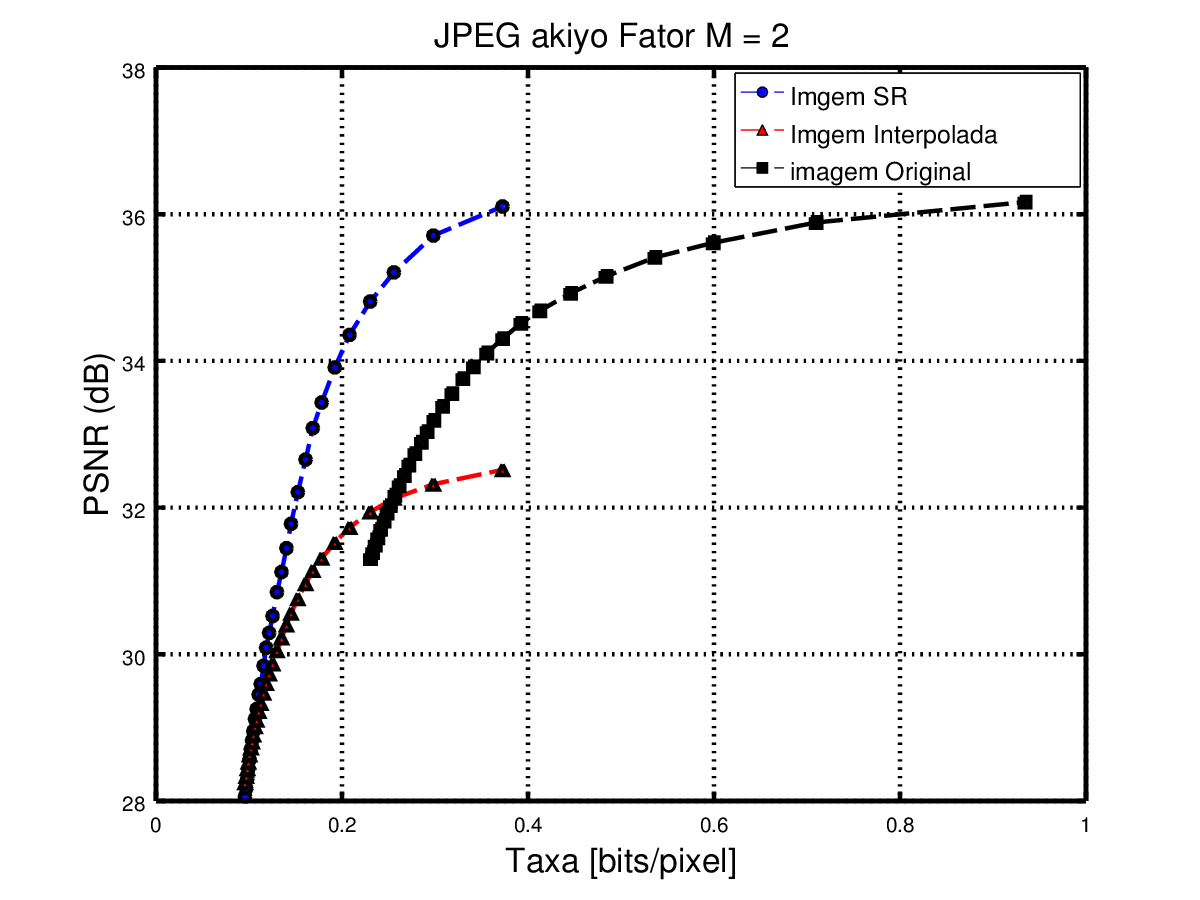
\includegraphics[scale=0.4]{figuras/JPEG_akiyo_Downsampling_factor_2.png}
	}
	\subfloat[]{
		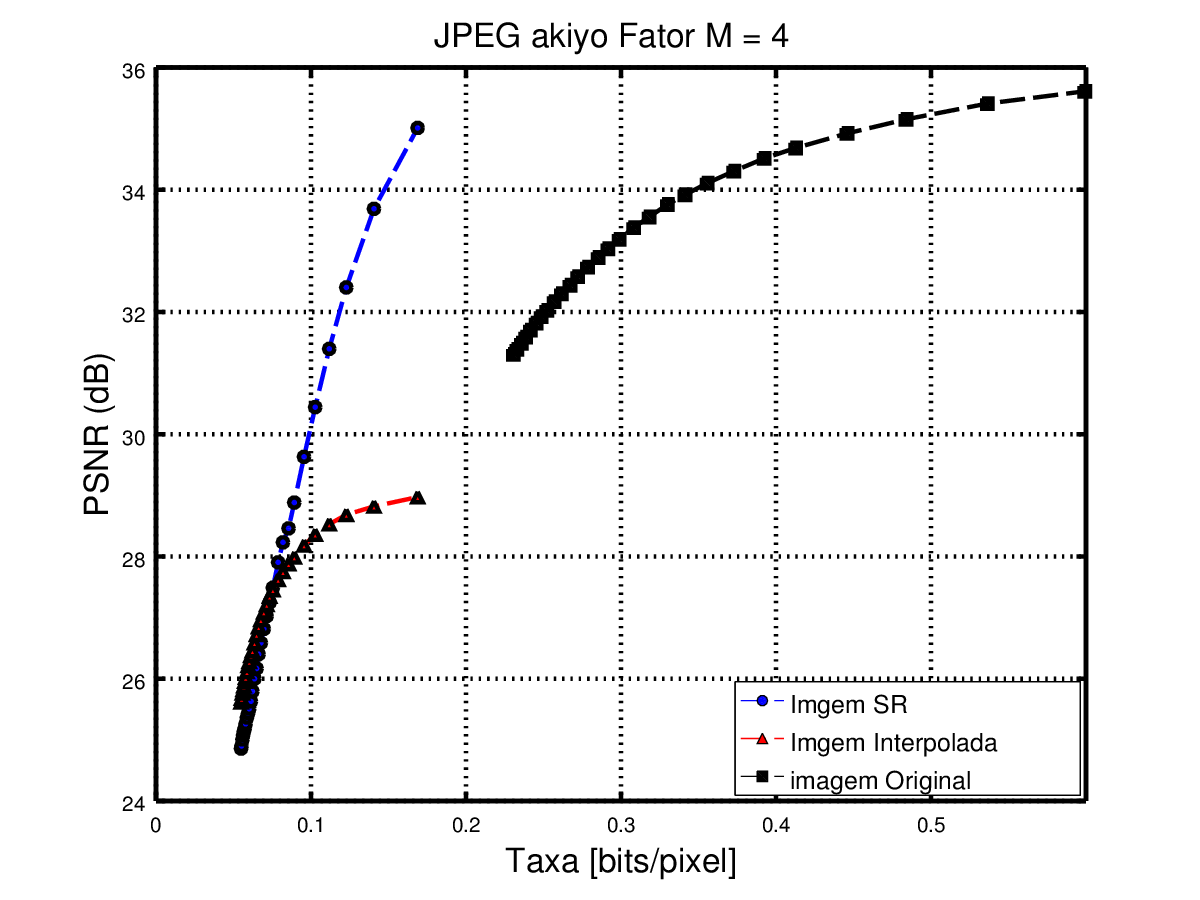
\includegraphics[scale=0.4]{figuras/JPEG_akiyo_Downsampling_factor_4.png}
	}
	\caption{Curva PSNR médio x Taxa, para a sequência de vídeo \textit{Akiyo}: (a)com um fator de decimação $M$ = 2, (b)com um fator de decimação $M$ = 4.}
	\label{fig:akiyo}
\end{figure}

Os gráficos das Figuras \ref{fig:football} e \ref{fig:akiyo}, incluem duas curvas de referência: a inferior que representa a qualidade dos quadros interpolados e a superior que representa a qualidade dos quadros originais ambos codificados pelo padrão JPEG. As curvas destas duas Figuras representam o comportamento característico das curvas geradas pelas oito sequências de vídeo testadas. As sequências de vídeo mais estáticas como \textit{Akiyo} e \textit{Carphone} apresentaram os melhores resultados, como esperado, consequentemente os maiores ganhos. As sequências que possuem um pouco mais de movimento como \textit{Foreman} e \textit{Crew} obtiveram resultados satisfatórios. Para as sequências que apresentam muito movimento e a várias entradas de novos elementos nas cenas, como \textit{Mobile} e \textit{Flower}, obteu-se resultados mais sigelos, mas que ainda assim são melhores que os dos quadros interpolados.

\begin{table}[hbt]
\centering
\caption{Tabela de ganhos médios para sequências codificas no padrão JPEG com fator de decimação $M$ = 2.}
\label{GanhoJpeg2}
\begin{tabular}{l|c}
\hline
\multicolumn{2}{c}{\textbf{Tabela de Ganhos}}\\
\hline
\hline
\multicolumn{2}{c}{\textbf{Para fator de decimação $M$ = 2}}\\
\hline
\hline			
Sequência	    & Ganho (dB)\\
\hline
\hline
\textit{Akiyo}		&2.0724\\
\hline
\textit{Foreman}		&1.5590\\
\hline
\textit{Bowing}		&1.6443\\
\hline
\textit{Carphone}		&1.8277\\
\hline
\textit{Crew}		&1.7288\\
\hline
\textit{Flower}		&1.3928\\
\hline
\textit{Football}		&1.5712\\
\hline
\textit{Mobile}	&1.2845\\
\hline
\hline
Média		&1.6351\\
\hline
\end{tabular}

\end{table}

\begin{table}[hbt]
\centering
\caption{Tabela de ganhos médios para sequências codificas no padrão JPEG com fator de decimação $M$ = 4.}	
\label{GanhoJpeg4}
\begin{tabular}{l|c}
\hline
\multicolumn{2}{c}{\textbf{Tabela de Ganhos}}\\
\hline
\hline
\multicolumn{2}{c}{\textbf{Para fator de decimação $M$ = 4}}\\
\hline
\hline			
Sequência	    & Ganho (dB)\\
\hline
\hline
\textit{Akiyo}		&2.1661\\
\hline
\textit{Foreman}		&1.5593 \\
\hline
\textit{Bowing}		&1.2851\\
\hline
\textit{Carphone}	& 2.0060\\
\hline
\textit{Crew}		& 1.9427\\
\hline
\textit{Flower}		&1.2137\\
\hline
\textit{Football}		&1.5794\\
\hline
\textit{Mobile}	&1.0615\\
\hline
\hline
Média	&1.0617\\
\hline
\end{tabular}
\end{table}
\subsection{Teste com codificação H.264/AVC}

A fim de avaliar o desempenho do algoritmo proposto, sobre o padrão H.264/AVC, aplicou-se ao algoritmo sequências de vídeo codificadas dentre as seguintes condições:
\begin{itemize}
 \setlength\itemsep{1cm}
\item[•] Cada sequência foi codificada separadamente utilizando o padrão H.264, em resolução mista. 
\item[•] Aplicou-se valores de 16 a 51 ao parâmetro  \textit{qp}, a faixa permitida pelo \textit{software} utilizado para implementação do padrão é de 0 a 51, sendo que 0 gera a codificação de melhor qualidade. Notou-se que utilizando os parâmetros de 0 a 15, a sequência decodificada tende a sequência original de tal forma que o cálculo do PSNR tende a infinito devido a limitação numérica da máquina utilizada, o que não é interessante para a abordagem do teste e por isso essa sequência de parâmetros foi desprezada. 
\item[•] Utilizou-se o \textit{framework ffmpeg}, especialmente a biblioteca \textit{libx264} para implementar a codificação no padrão H.264.
\item[•] Assim como para o padrão JPEG, foi considerada somente as taxas dos quadros em baixa resolução. Utilizou-se os mesmos tamanhos de janela e macroblocos que para o padrão JPEG.
\item[•] Calculou-se os ganhos médios \cite{bjontegaard2001calcuation} de qualidade (PSNR) para o algoritmo proposto em relação aos quadros interpolados. Estes resultados são ilustrados nas Tabelas \ref{GanhoH2642} e \ref{GanhoH2644}.
\end{itemize}

\begin{table}[hbt]
\centering
\caption{Tabela de ganhos médios para sequências codificas no padrão H.264 com fator de decimação $M$ = 2.}
\label{GanhoH2642}
\begin{tabular}{l|c}
\hline
\multicolumn{2}{c}{\textbf{Tabela de Ganhos}}\\
\hline
\hline
\multicolumn{2}{c}{\textbf{Para fator de decimação $M$ = 2}}\\
\hline
\hline			
Sequência	    & Ganho (dB)\\
\hline
\hline
\textit{Akiyo}		&3.2273\\
\hline
\textit{Foreman}		&2.0085\\
\hline
\textit{Bowing}		&2.5412\\
\hline
\textit{Carphone}	&2.4535\\
\hline
\textit{Crew}		&2.5024\\
\hline
\textit{Flower}		&1.8606\\
\hline
\textit{Football}	&2.3817\\
\hline
\textit{Mobile}	&1.8949\\
\hline
\hline
Média		&2.3587\\
\hline
\end{tabular}

\end{table}

\begin{table}[hbt]
\centering
\caption{Tabela de ganhos médios para sequências codificas no padrão H.264 com fator de decimação $M$ = 4.}	
\label{GanhoH2644}
\begin{tabular}{l|c}
\hline
\multicolumn{2}{c}{\textbf{Tabela de Ganhos}}\\
\hline
\hline
\multicolumn{2}{c}{\textbf{Para fator de decimação $M$ = 4}}\\
\hline
\hline			
Sequência	    & Ganho (dB)\\
\hline
\hline
\textit{Akiyo}		&2.2735\\
\hline
\textit{Foreman}		&1.6583 \\
\hline
\textit{Bowing}		&2.0681\\
\hline
\textit{Carphone}	& 2.0180\\
\hline
\textit{Crew}		& 2.0091\\
\hline
\textit{Flower}		&1.5670\\
\hline
\textit{Football}	&2.0459\\
\hline
\textit{Mobile}	&1.7302\\
\hline
\hline
Média	&1.9213\\
\hline
\end{tabular}
\end{table}

As Figuras \ref{fig:footballh264} e \ref{fig:akiyoh264} apresentam o desempenho da super-resolução proposta em termos de taxa e distorção para as sequêcias \textit{Football} e \textit{Akiyo} respectivamente. Estas curvas são representativas do comportamento típico das sequências testadas. Assim, verificou-se uma diferença no desmpenho do algoritmo de acordo com o nível do escalonamento aplicado as quadros interpolados e de referência. Notou-se também que para taxas mais baixas, a qualidade dos quadros super-resolvidos é superior a dos quadros originas degradados apenas pelo codificação, o que já justifica a aplicação da técnica proposta.


\begin{figure}[H]
	\centering
    \subfloat[]{
    	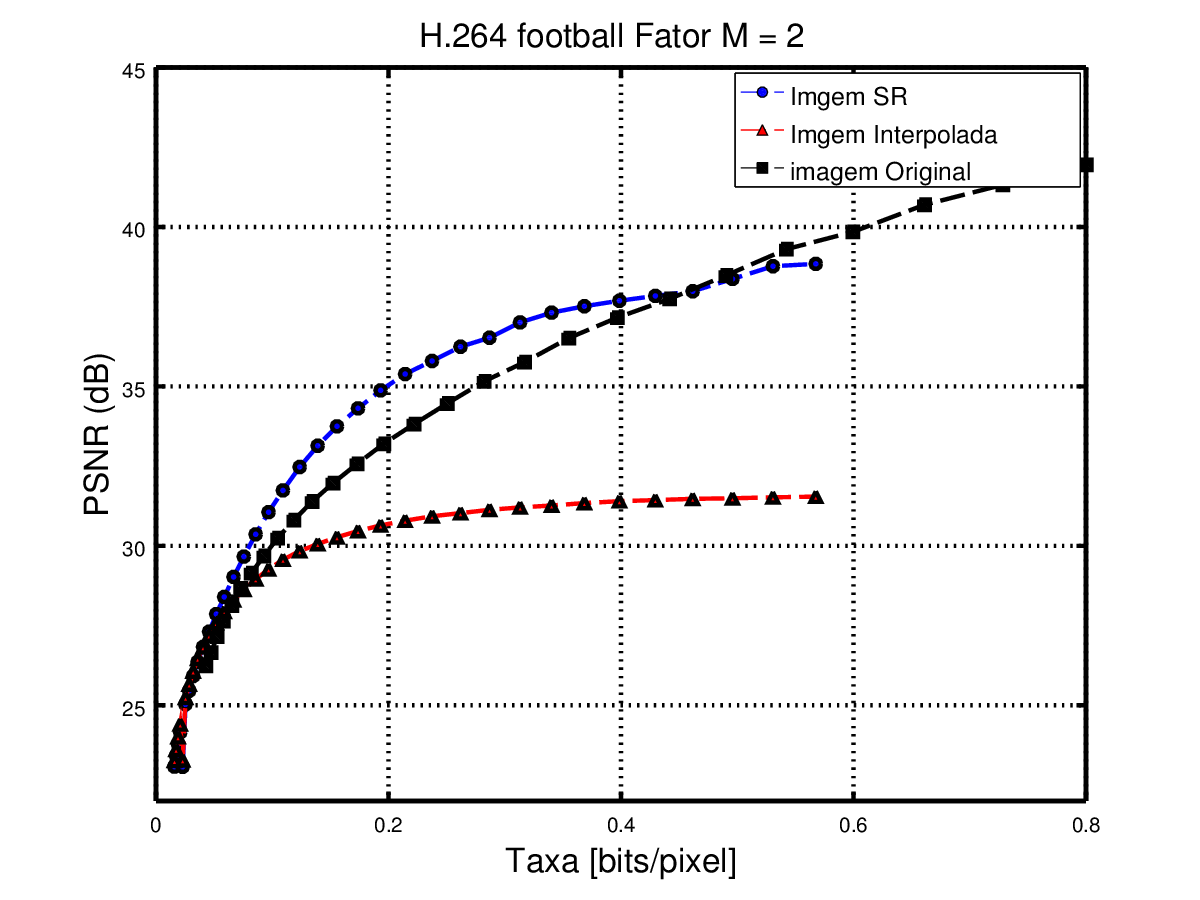
\includegraphics[scale=0.4]{figuras/H264_football_Downsampling_factor_2.png}
    }
        \subfloat[]{
    	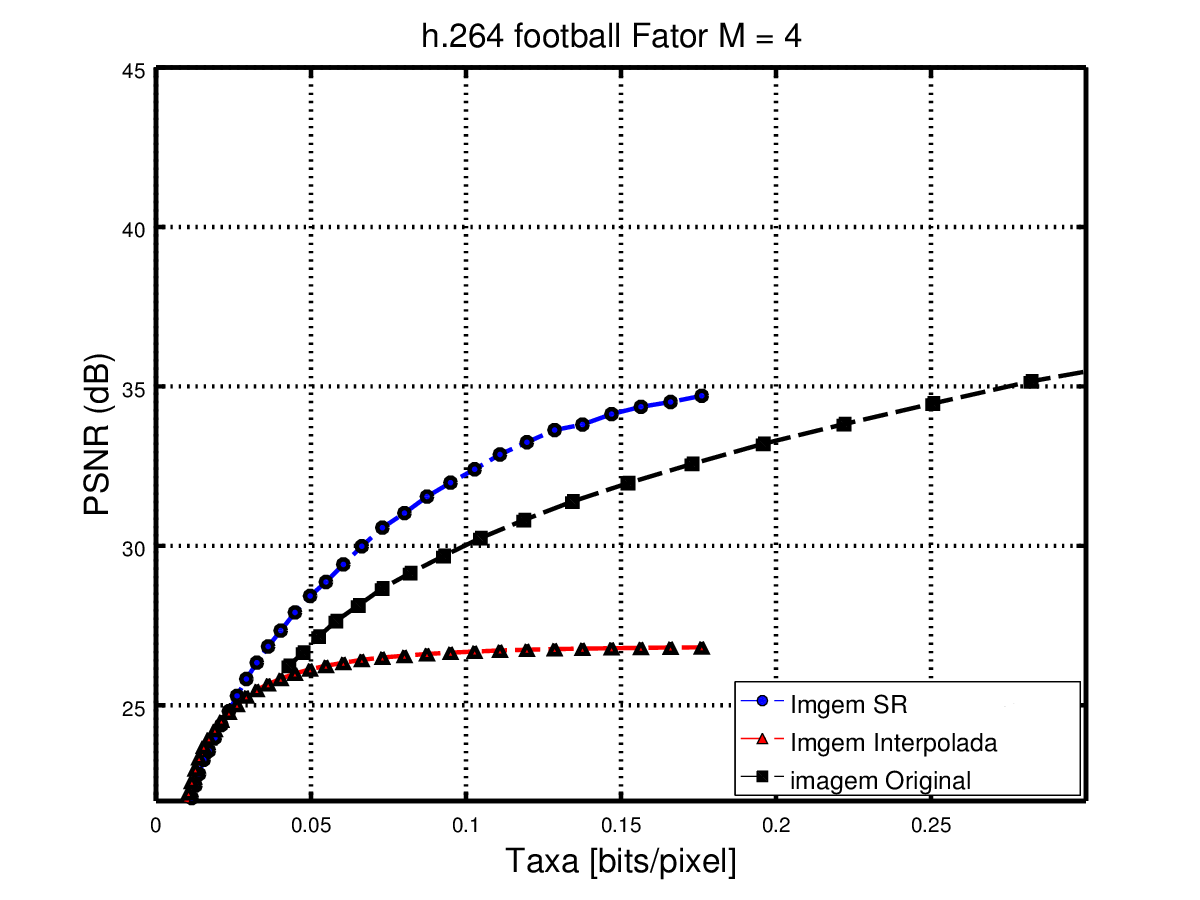
\includegraphics[scale=0.4]{figuras/H264_football_Downsampling_factor_4.png}
    }
	\caption{Curva PSNR médio x Taxa, para a sequência de vídeo \textit{Football}: (a) com um fator de decimação $M$ = 2, (b) com um fator de decimação $M$ = 4.}
	\label{fig:footballh264}
\end{figure}


\begin{figure}[H]
	\centering
	\subfloat[]{
	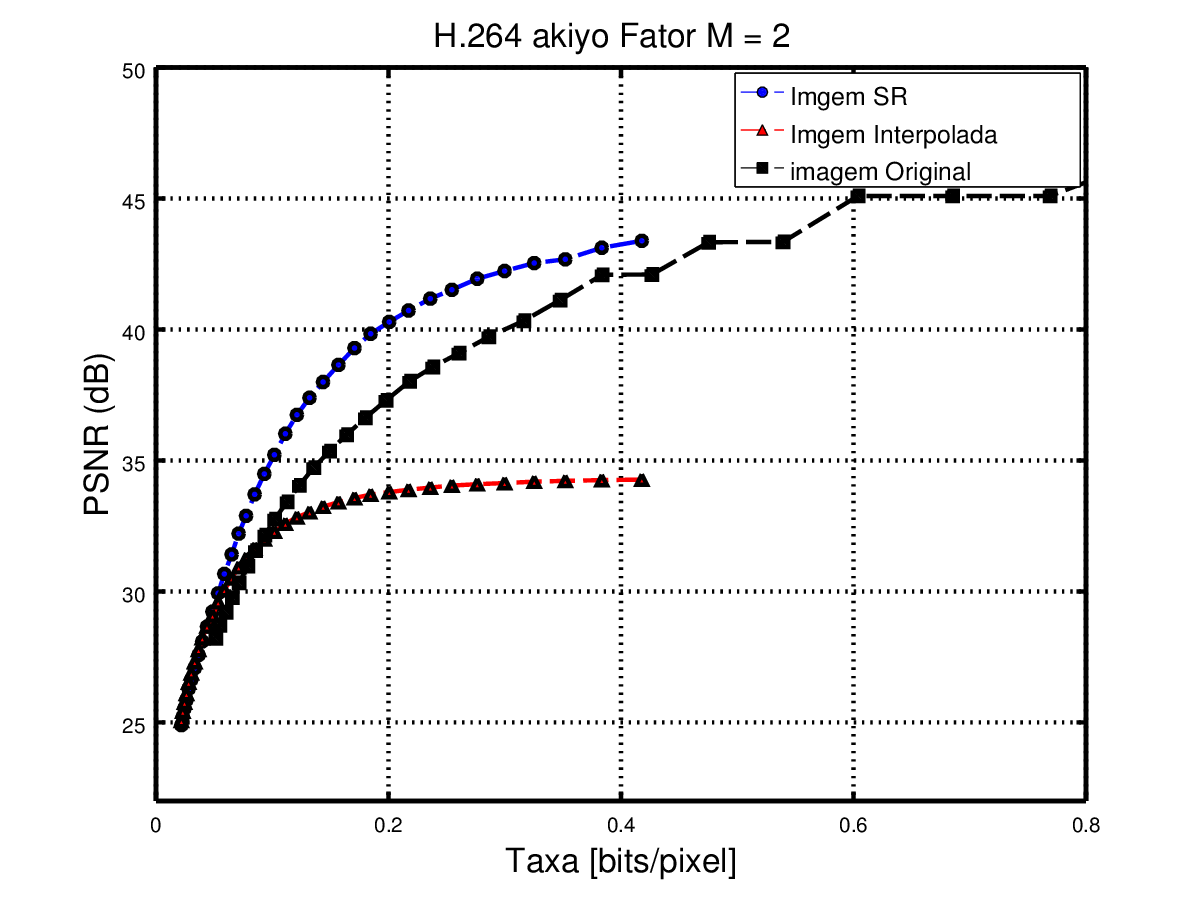
\includegraphics[scale=0.4]{figuras/H264_akiyo_Downsampling_factor_2.png}
    }
    \subfloat[]{
	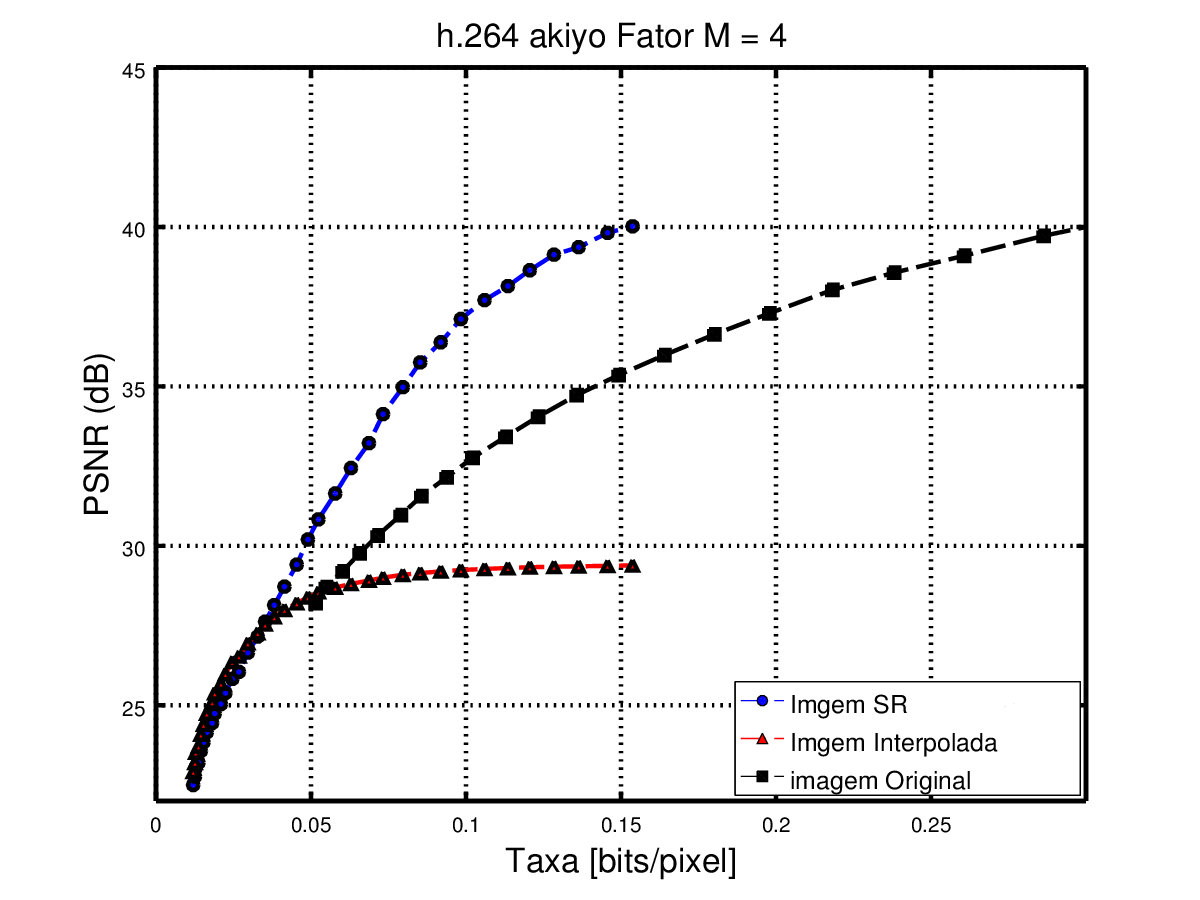
\includegraphics[scale=0.4]{figuras/H264_akiyo_Downsampling_factor_4.png}
    }
	\caption{Curva PSNR médio x Taxa, para a sequência de vídeo \textit{Akiyo}: (a)com um fator de decimação $M$ = 2, (b)com um fator de decimação $M$ = 4.}
	\label{fig:akiyoh264}
\end{figure}
\clearpage
\subsection{Resultados Subjetivos}

Observando as imagens desta Seção, pode-se perceber que mesmo para as sequências de vídeo com grande quantidade de movimento e novos elementos a cada cena, as imagens super-resolvidas são apresentadas sem detalhes visualmente incômodos. 

Em geral as bordas, letras, algumas texturas e detalhes são difíceis de se ver nos quadros interpolados, no entanto ficam claramente visíveis nos quadros super-resolvidos, o que mostra que as informações de alta frequência adicionadas aos quadros interpolados possuem um bom \textit{mathing}. 
\clearpage
\subsection{Teste com codificação JPEG}
\begin{figure}[H]
    \centering
    \subfloat[]{
	    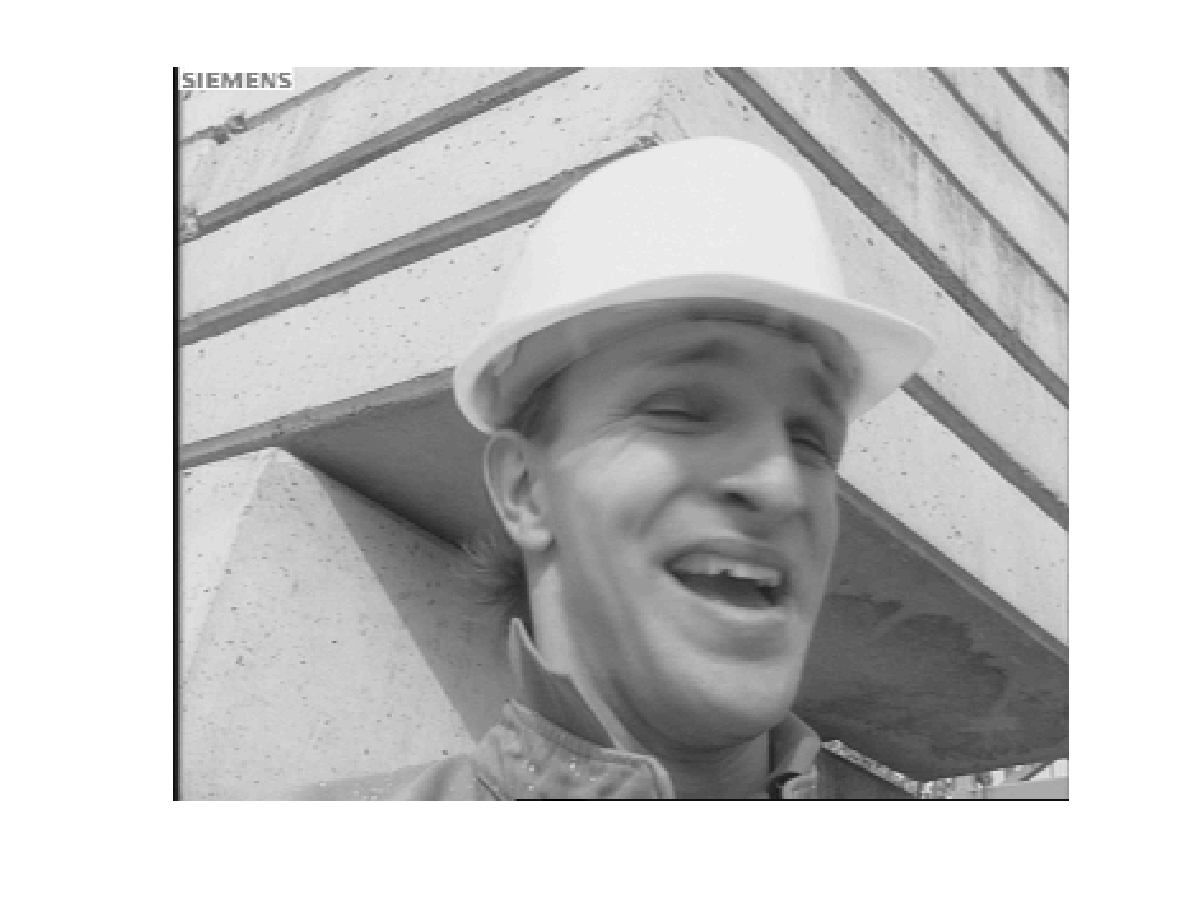
\includegraphics[width=0.5\linewidth]{figuras/foreman_original.png}
    }
    \qquad
    \subfloat[]{
    	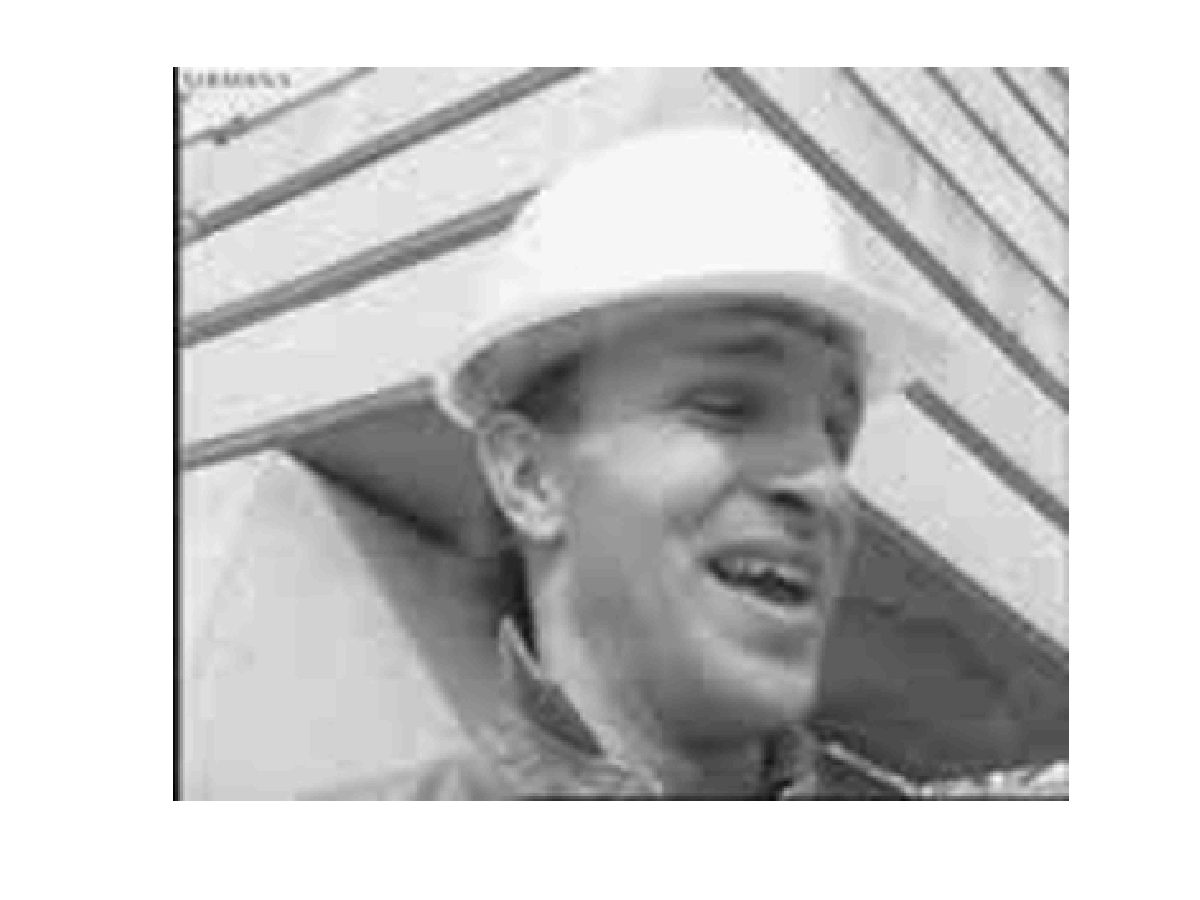
\includegraphics[width=0.5\linewidth]{figuras/foreman_interbolada.png}
    }
	\qquad
    \subfloat[]{
    	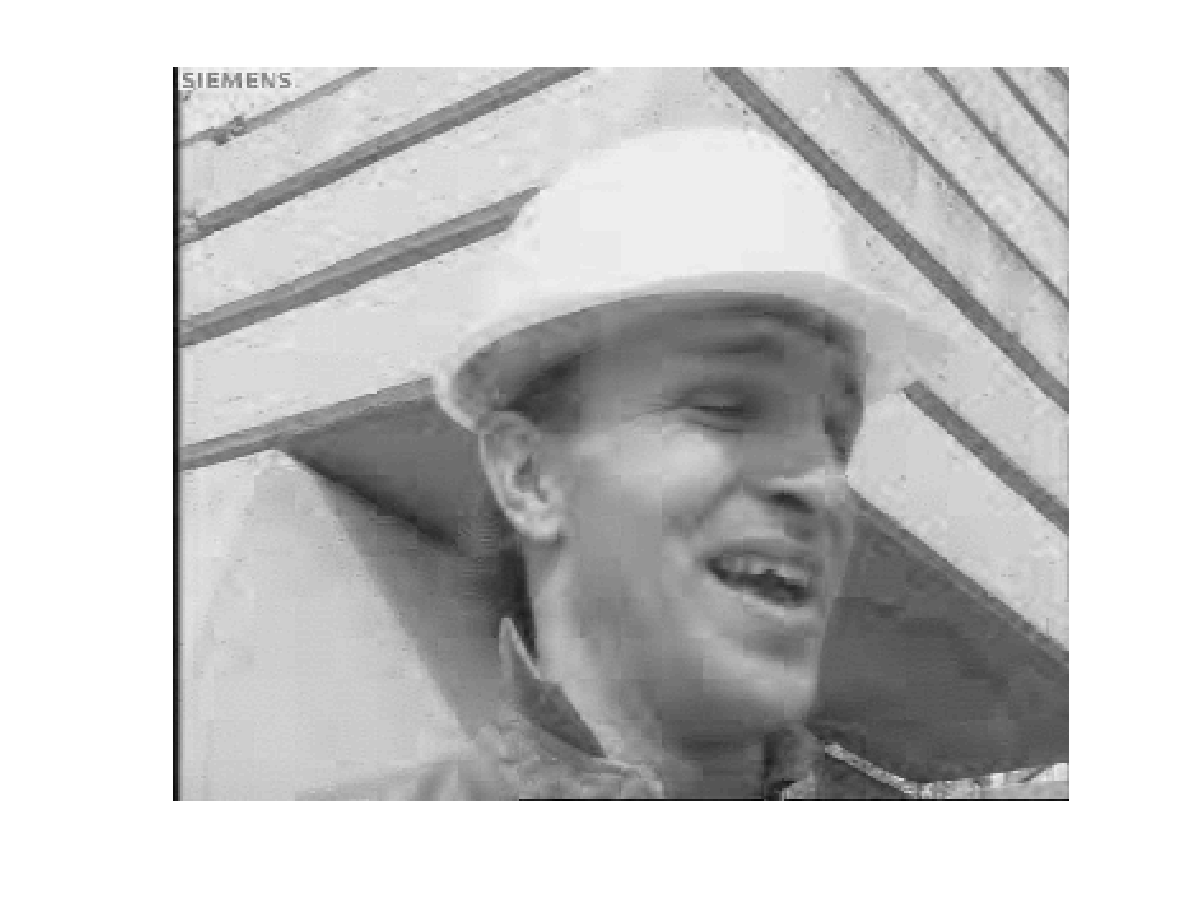
\includegraphics[width=0.5\linewidth]{figuras/foreman_SP.png}
    }

    \caption{\textit{Foreman} - Quadro 6, $M = 2$, \textit{Qscale} = 10 : (a) Imagem Original, (b)Imagem Interpolada (PSNR = 21.950 dB), (c)Imagem Super-resolvida (PSNR = 21.776 dB).}
	    
    \label{fig:1}
\end{figure}

\begin{figure}[H]
    \centering
    \subfloat[]{
	    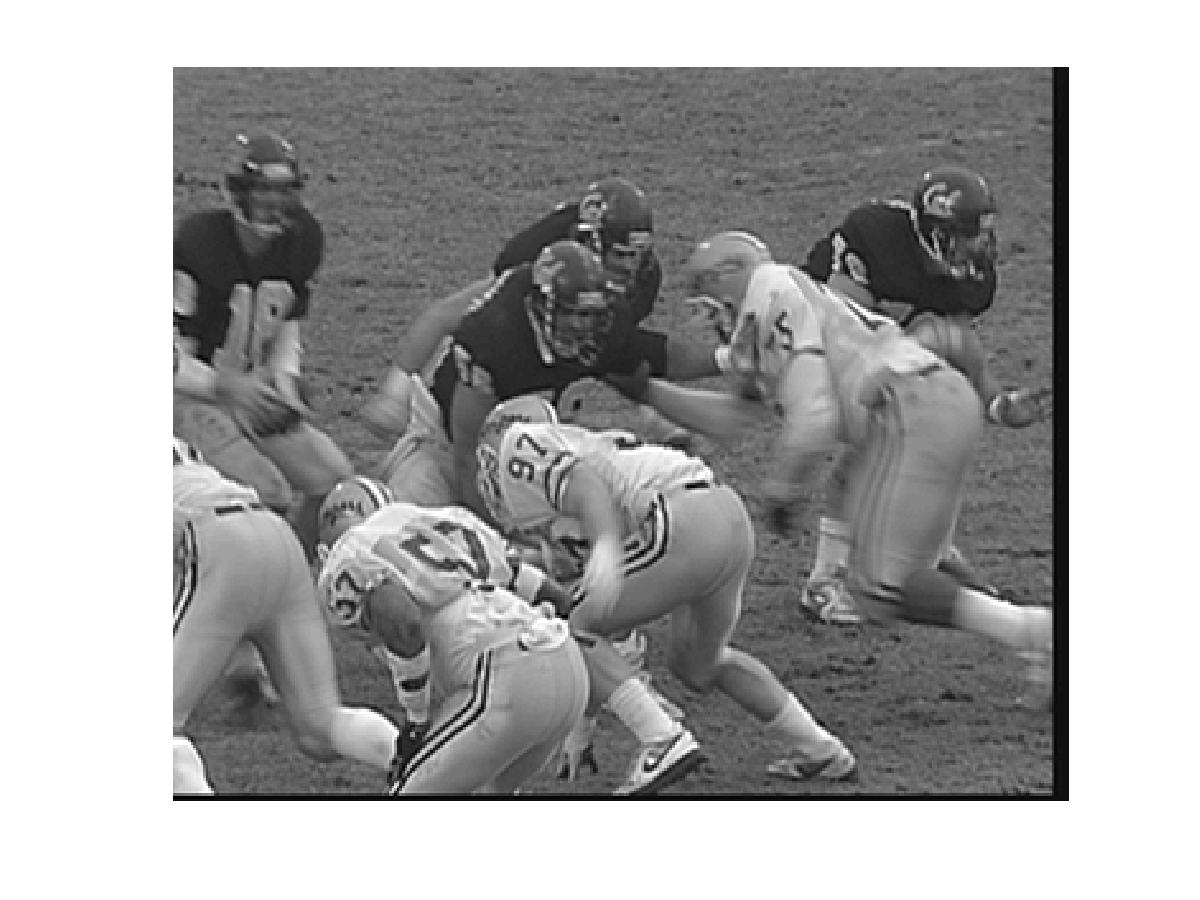
\includegraphics[width=0.5\linewidth]{figuras/football_original.png}
    }
    \qquad
    \subfloat[]{
    	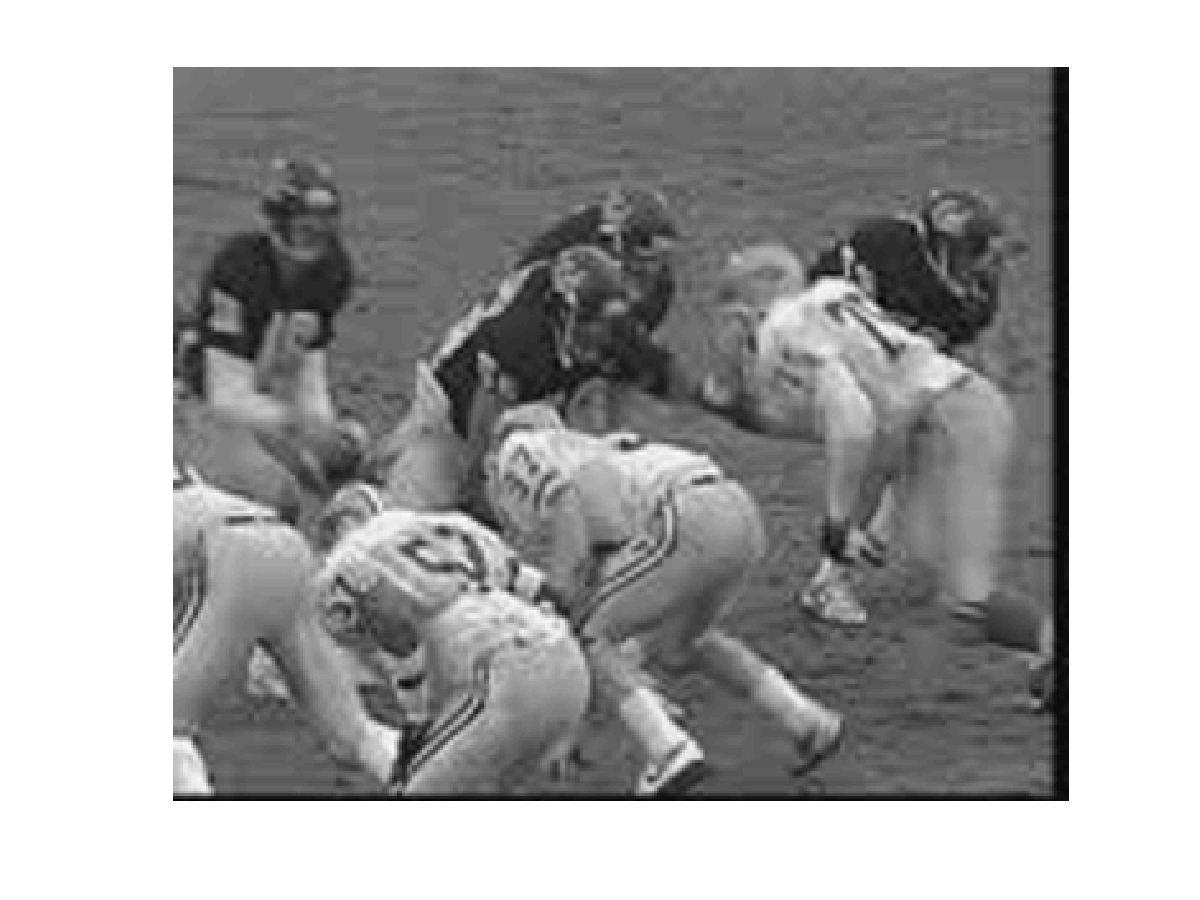
\includegraphics[width=0.5\linewidth]{figuras/football_interbolada.png}
    }
	
    \subfloat[]{
    	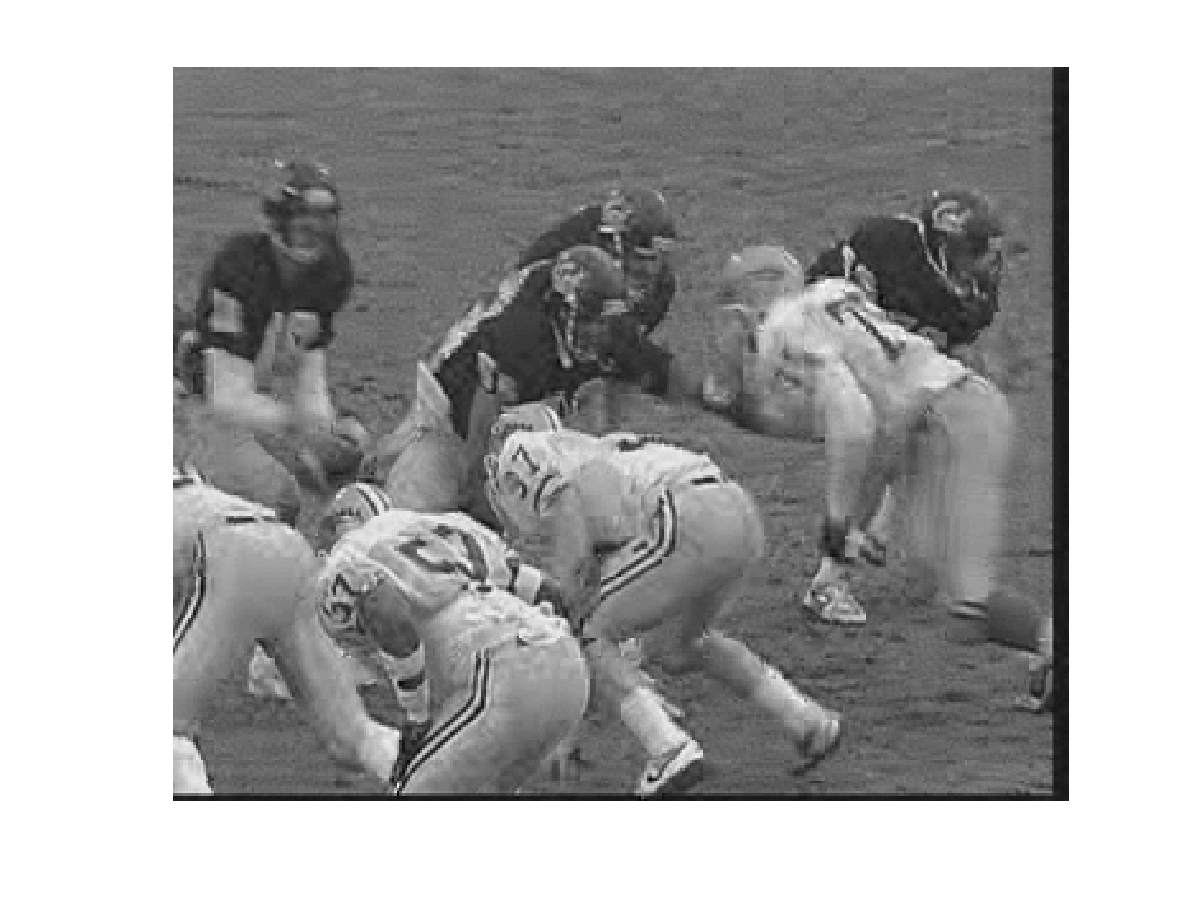
\includegraphics[width=0.5\linewidth]{figuras/football_SP.png}
    }

    \caption{\textit{Football} - Quadro 4, $M = 2$, \textit{Qscale} = 10 : (a) Imagem Original, (b)Imagem Interpolada (PSNR = 16.847 dB), (c)Imagem Super-resolvida (PSNR = 17.176 dB).}
	    
    \label{fig:2}
\end{figure}

\begin{figure}[H]
    \centering
    \subfloat[]{
	    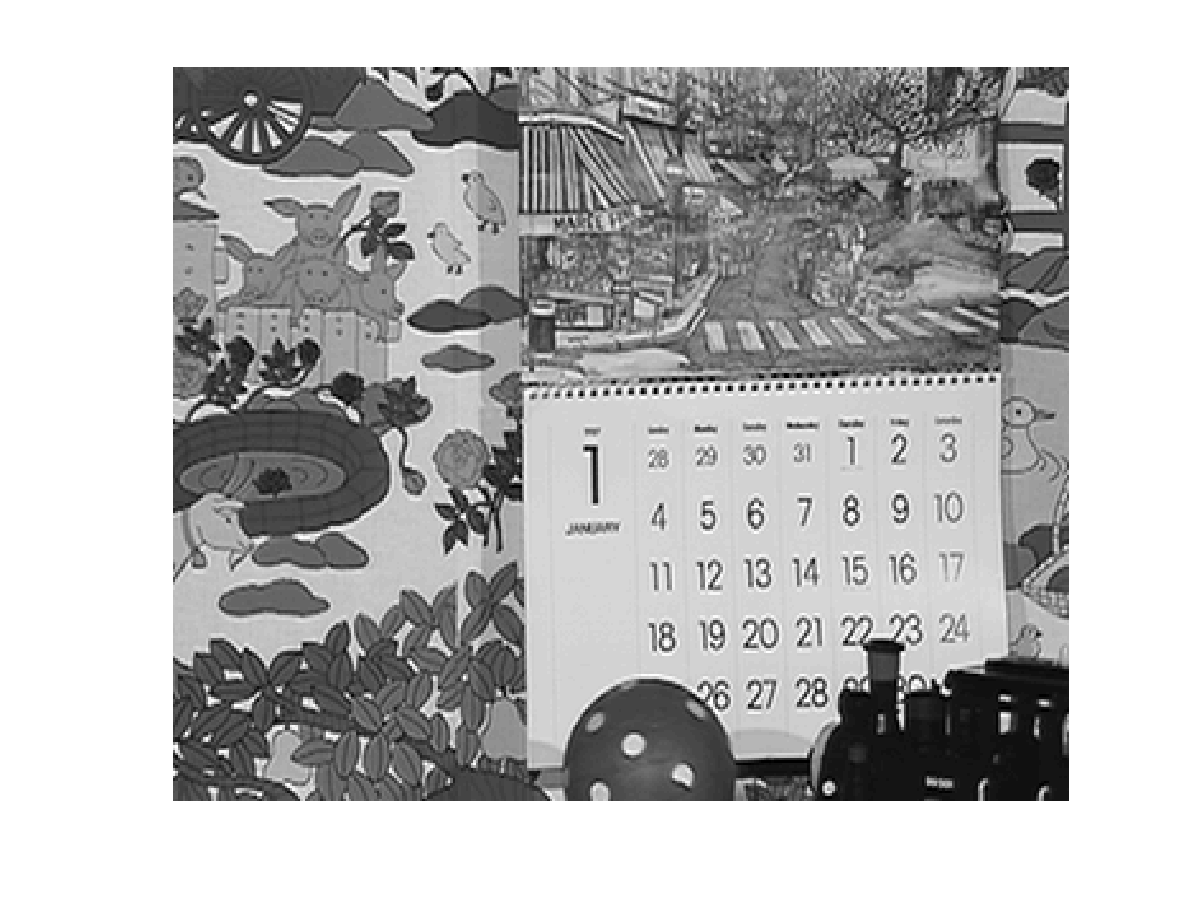
\includegraphics[width=0.5\linewidth]{figuras/mobile_original.png}
    }
    \qquad
    \subfloat[]{
    	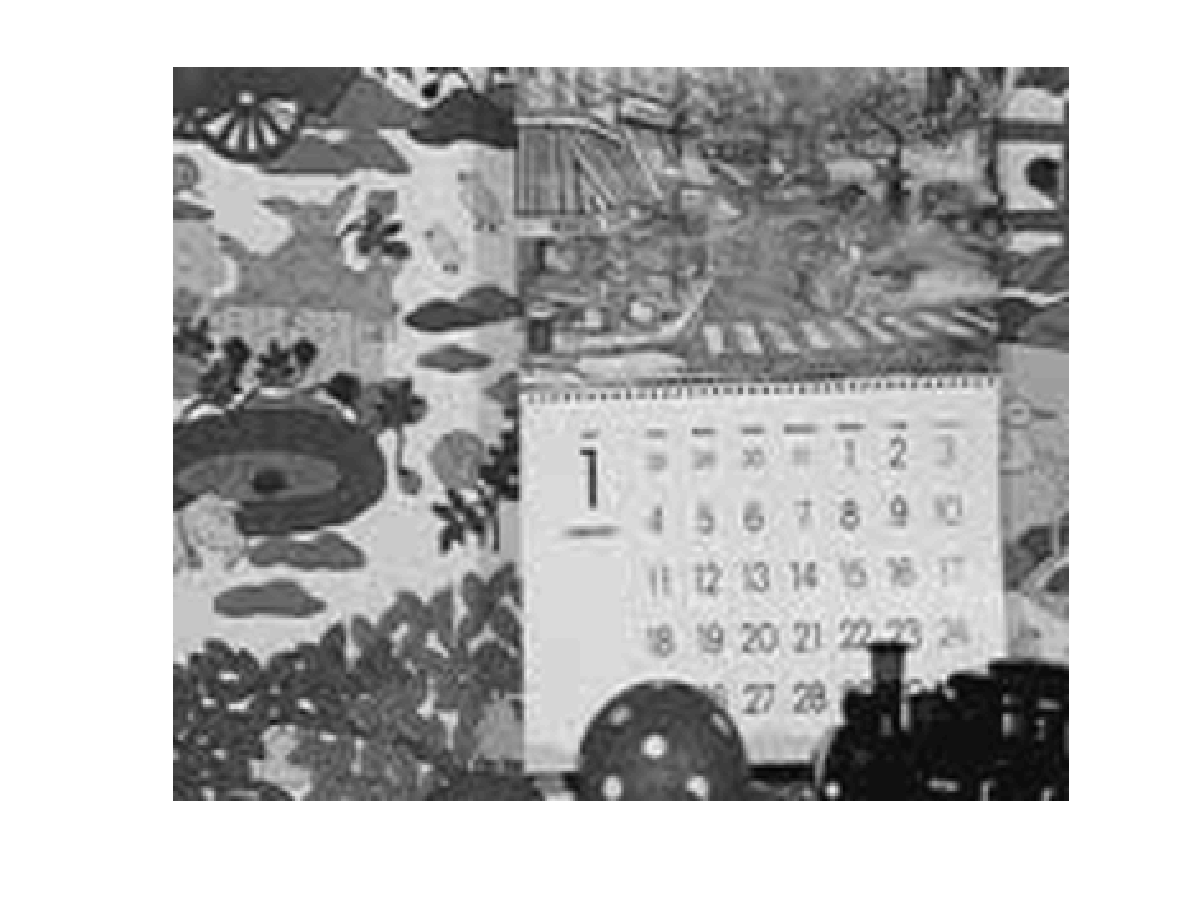
\includegraphics[width=0.5\linewidth]{figuras/mobile_interbolada.png}
    }
	
    \subfloat[]{
    	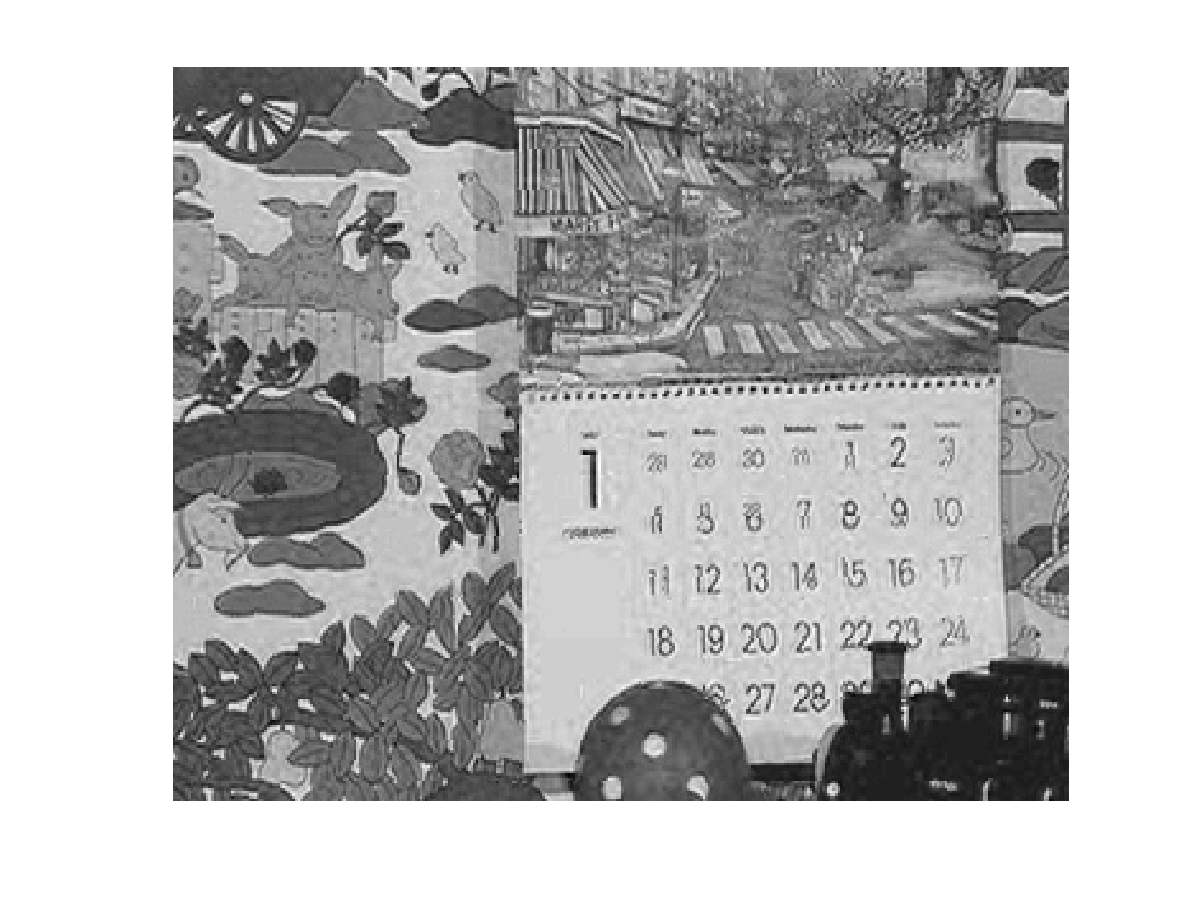
\includegraphics[width=0.5\linewidth]{figuras/mobile_SP.png}
    }

    \caption{\textit{Mobile} - Quadro 4, $M = 2$, \textit{Qscale} = 10 : (a) Imagem Original, (b)Imagem Interpolada (PSNR = 16.532 dB), (c)Imagem Super-resolvida (PSNR = 17.902 dB).}
	    
    \label{fig:3}
\end{figure}

\subsection{Teste com codificação H.264/AVC}
\begin{figure}[h]
    \centering
    \subfloat[]{
	    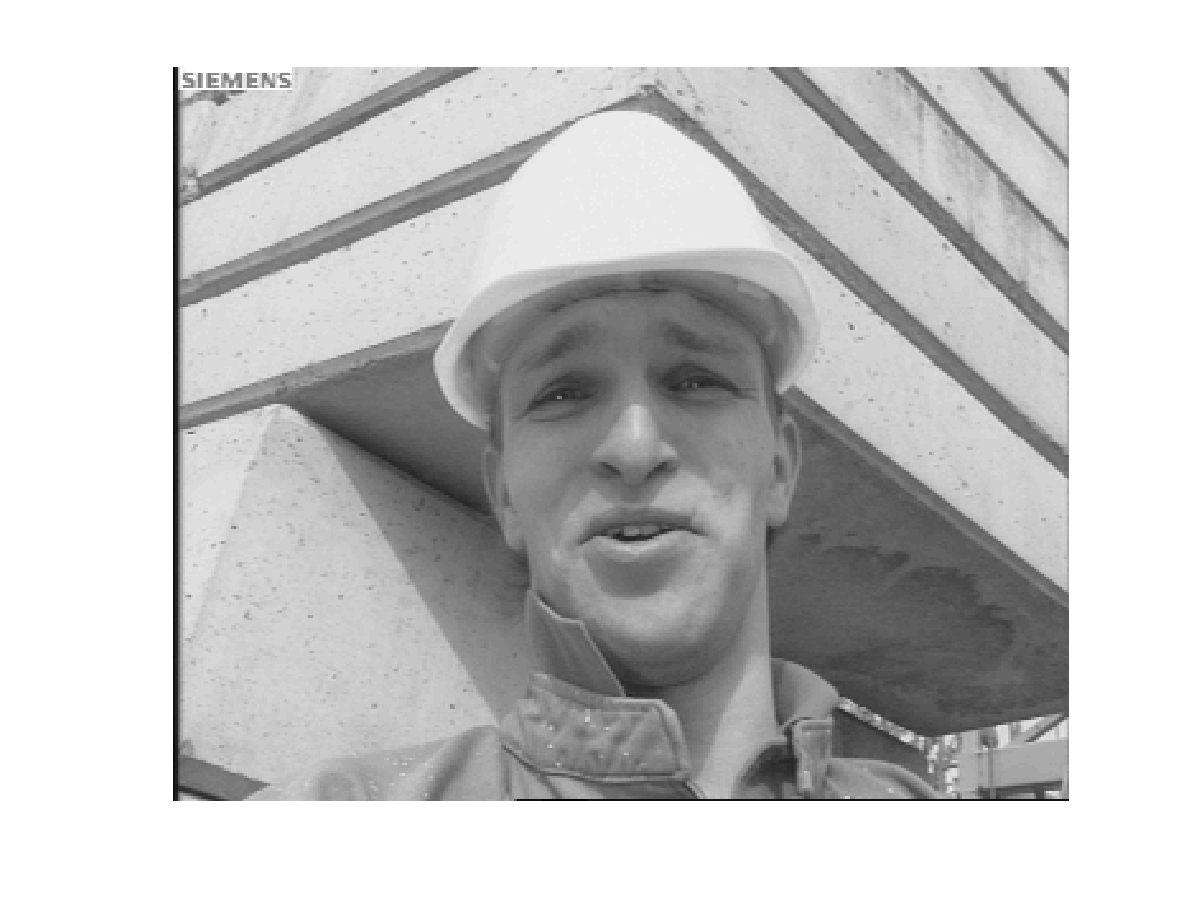
\includegraphics[width=0.5\linewidth]{figuras/foreman_original_h264.png}
    }
    \qquad
    \subfloat[]{
    	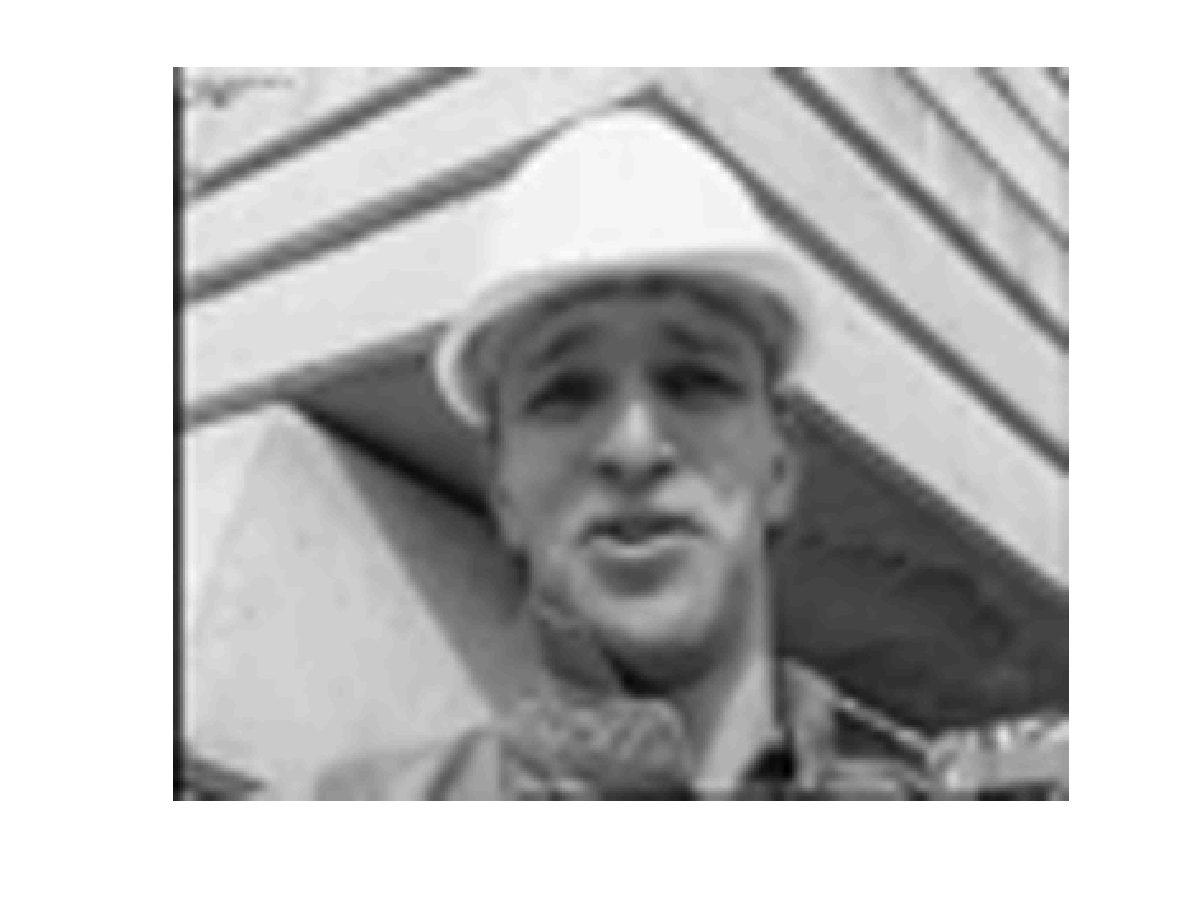
\includegraphics[width=0.5\linewidth]{figuras/foreman_interbolada_h264.png}
    }
	
    \subfloat[]{
    	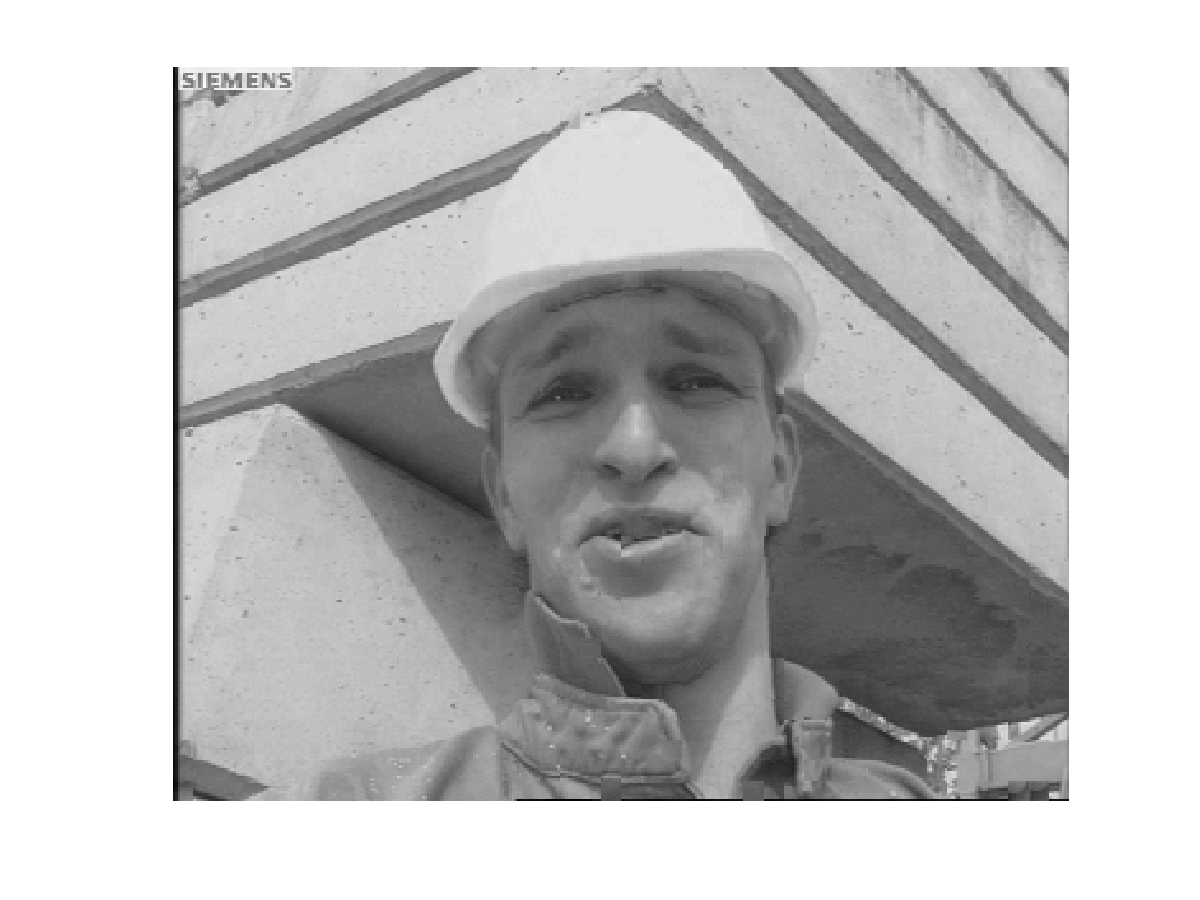
\includegraphics[width=0.5\linewidth]{figuras/foreman_SP_h264.png}
    }

    \caption{\textit{Foreman} - Quadro 30, $M = 2$, \textit{Qscale} = 10 : (a) Imagem Original, (b)Imagem Interpolada (PSNR = 26.399 dB), (c)Imagem Super-resolvida (PSNR = 31.503 dB).}
	    
    \label{fig:4}
\end{figure}

\begin{figure}[h]
    \centering
    \subfloat[]{
	    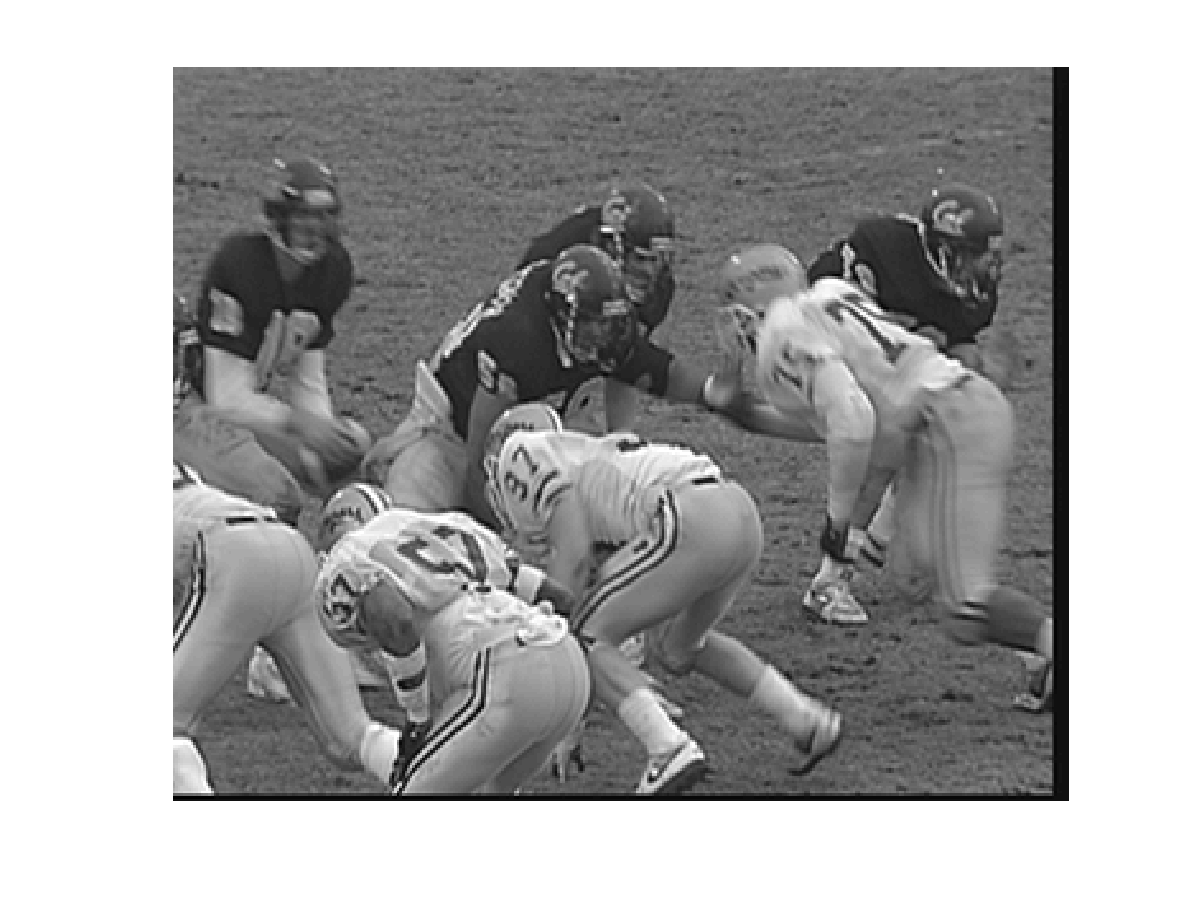
\includegraphics[width=0.5\linewidth]{figuras/football_original_h264.png}
    }
    \qquad
    \subfloat[]{
    	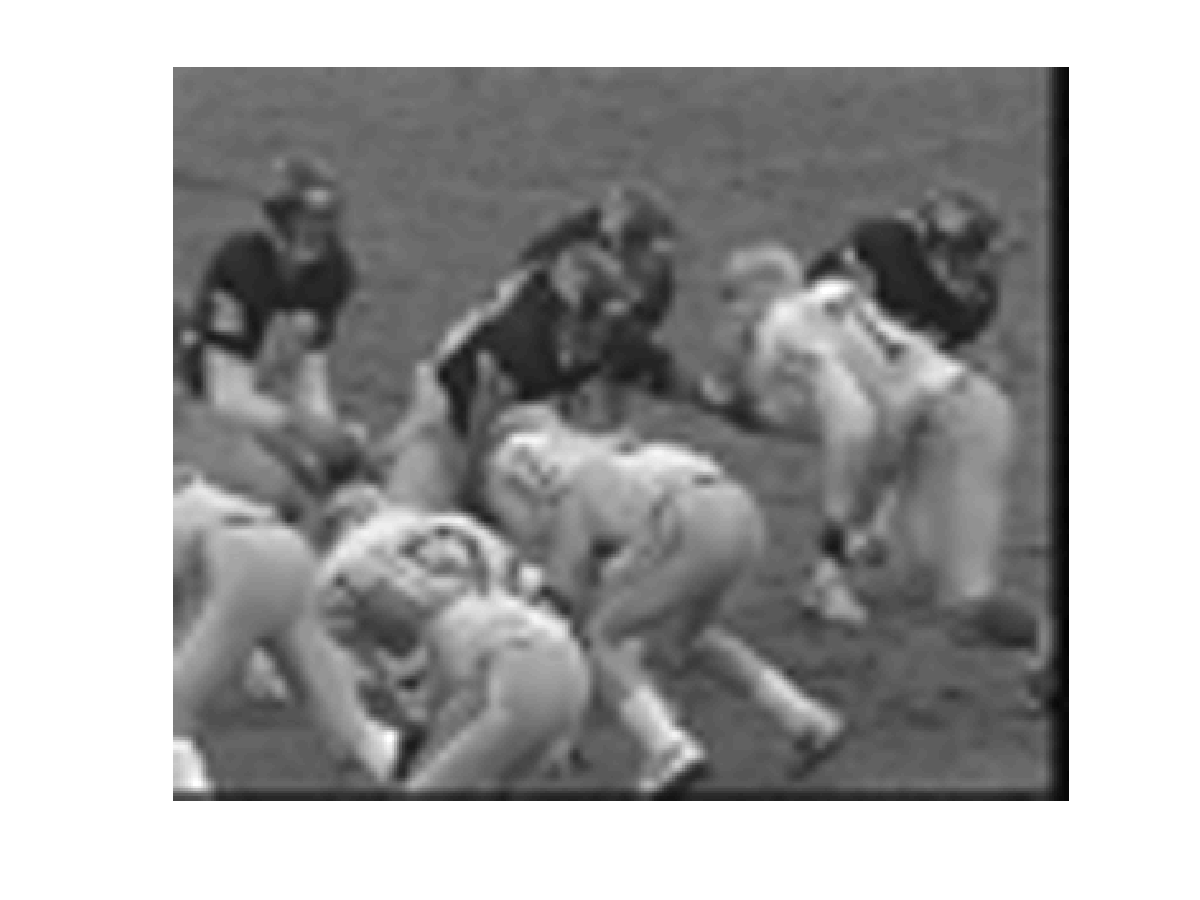
\includegraphics[width=0.5\linewidth]{figuras/football_interbolada_h264.png}
    }
	
    \subfloat[]{
    	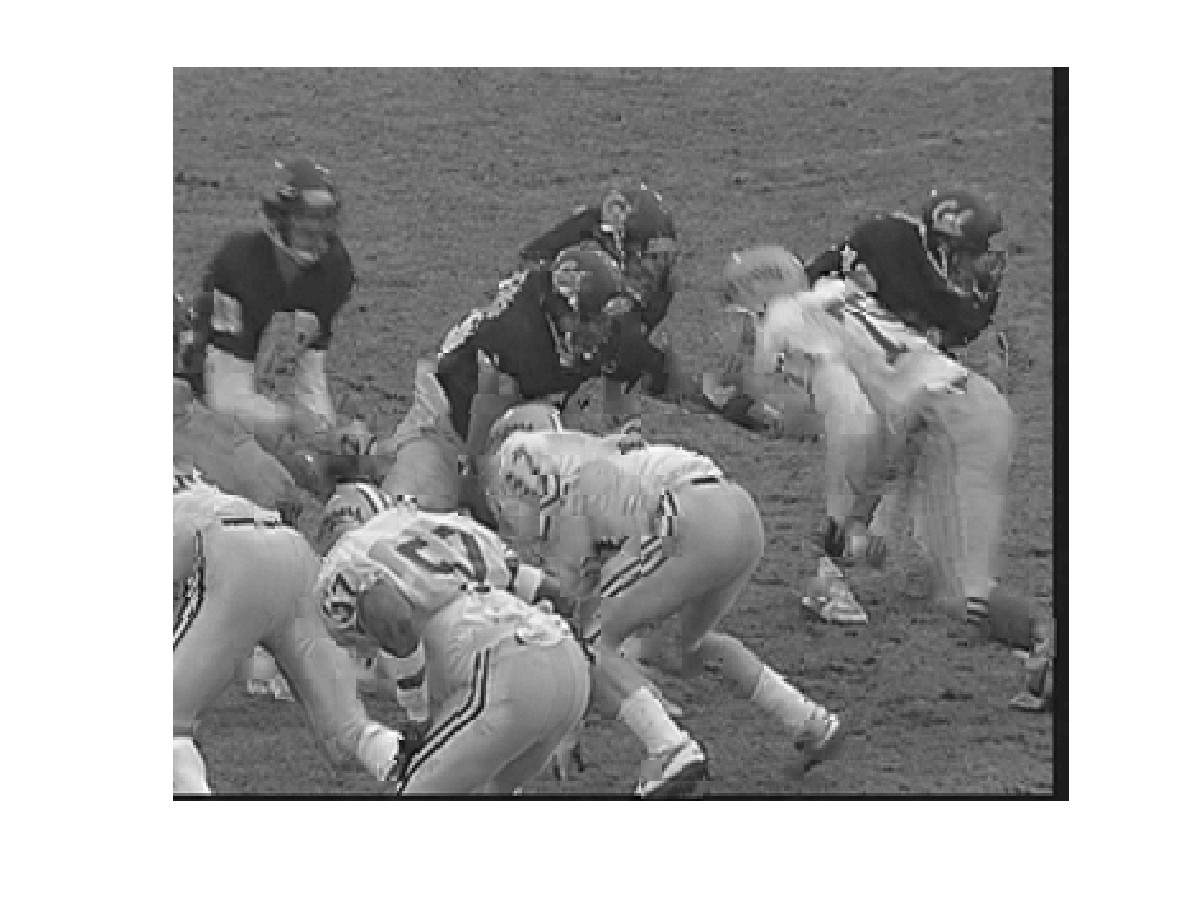
\includegraphics[width=0.5\linewidth]{figuras/football_SP_h264.png}
    }

    \caption{\textit{Football} - Quadro 3, $M = 2$, \textit{Qscale} = 10 : (a) Imagem Original, (b)Imagem Interpolada (PSNR = 22.946 dB), (c)Imagem Super-resolvida (PSNR = 24.286 dB).}
	    
    \label{fig:5}
\end{figure}

\begin{figure}[h]
    \centering
    \subfloat[]{
	    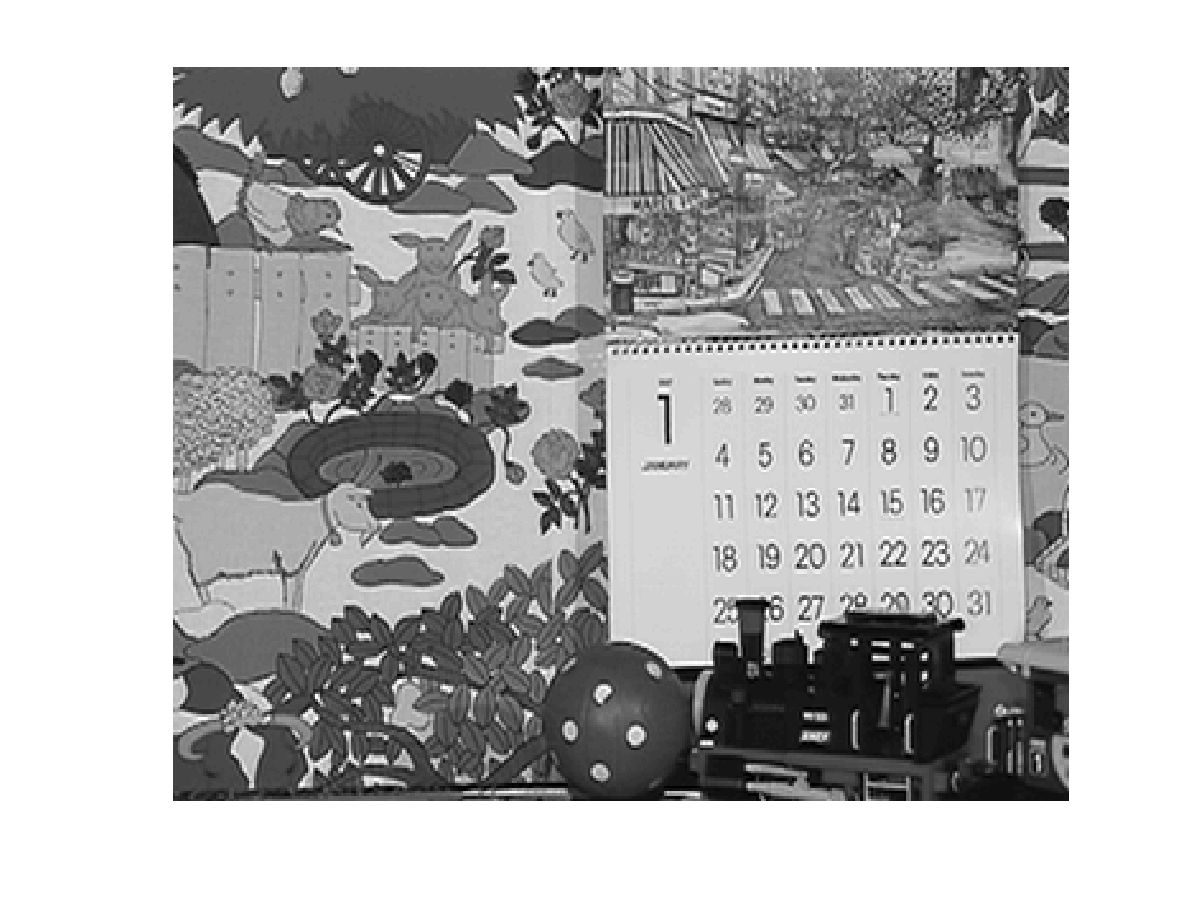
\includegraphics[width=0.5\linewidth]{figuras/mobile_original_h264.png}
    }
    \qquad
    \subfloat[]{
    	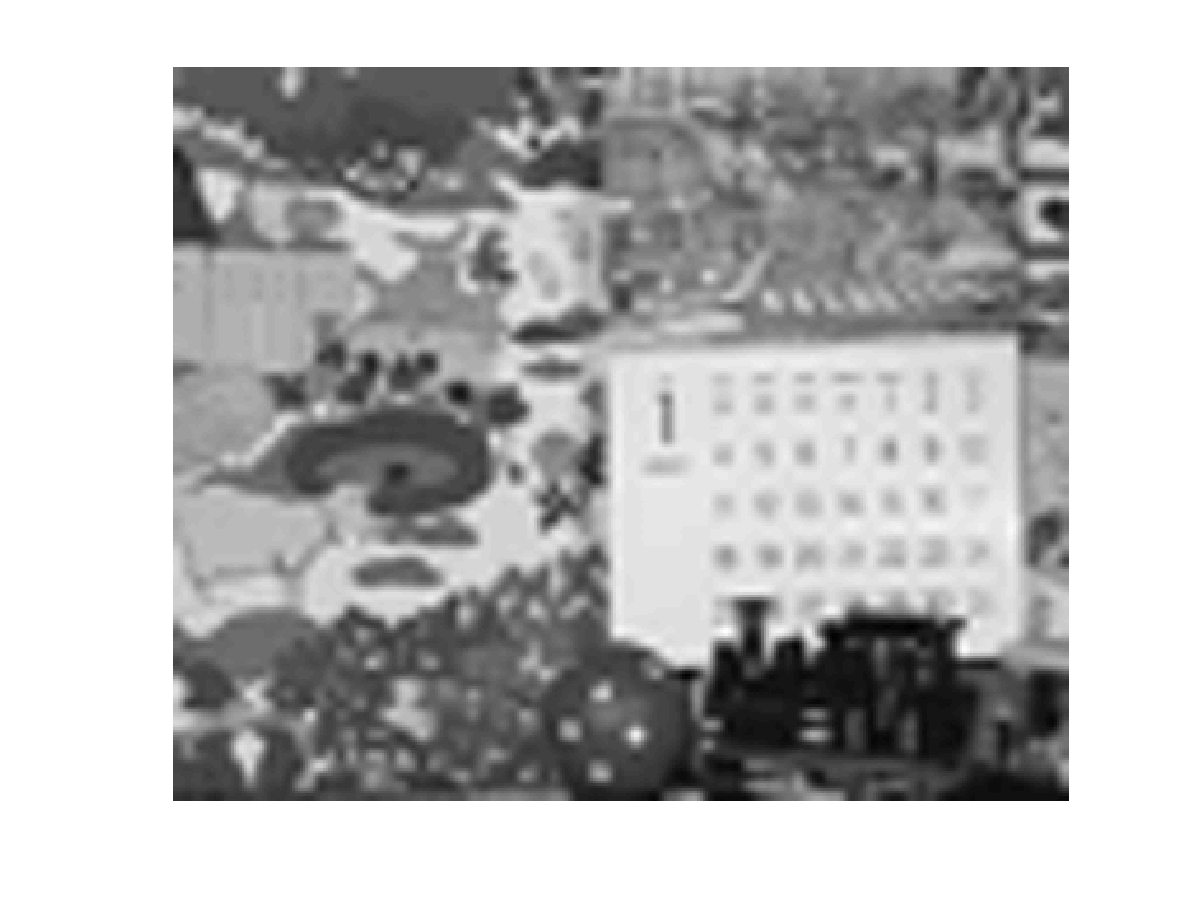
\includegraphics[width=0.5\linewidth]{figuras/mobile_interbolada_h264.png}
    }
    \qquad
    \subfloat[]{
    	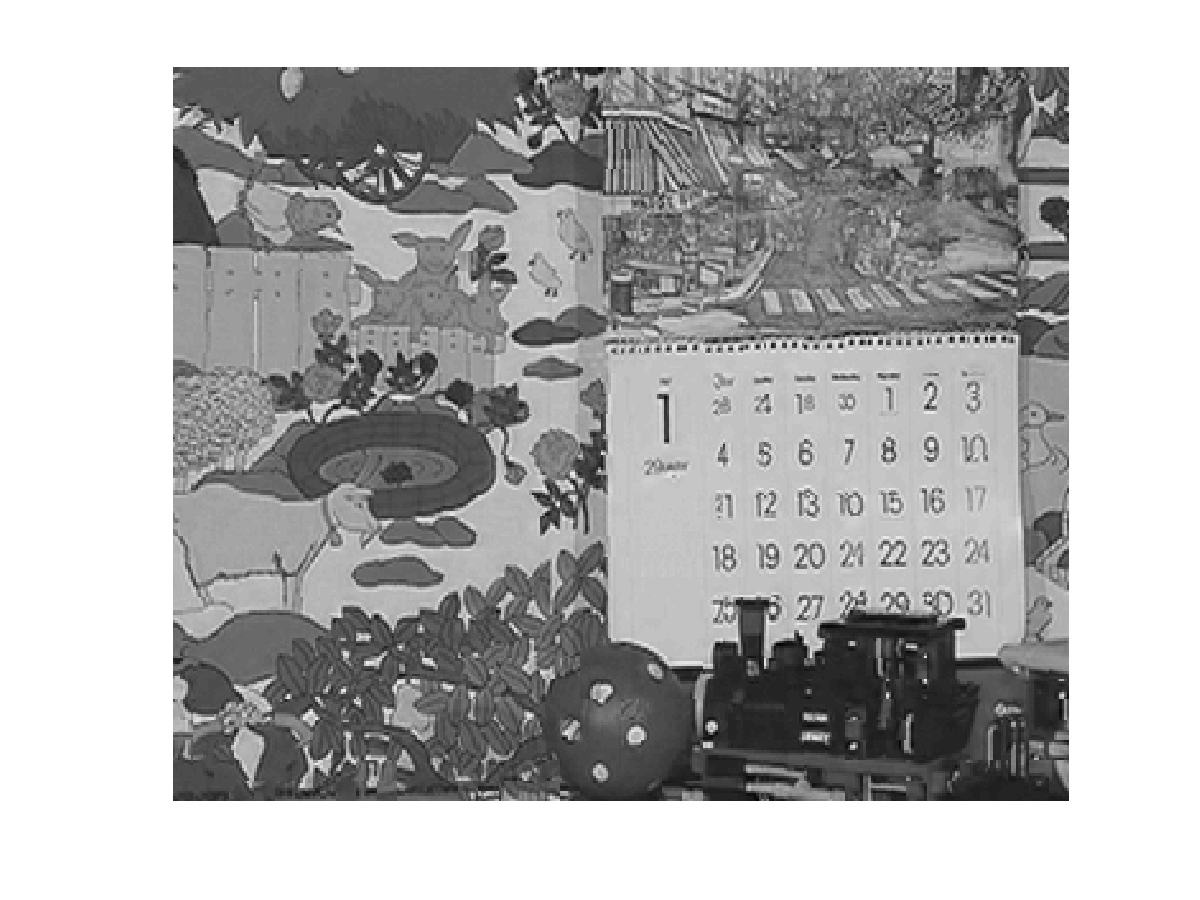
\includegraphics[width=0.5\linewidth]{figuras/mobile_SP_h264.png}
    }
    \caption{\textit{Mobile} - Quadro 33, $M = 2$, \textit{Qscale} = 10 : (a) Imagem Original, (b)Imagem Interpolada (PSNR = 18.756 dB), (c)Imagem Super-resolvida (PSNR = 21.211 dB).}
	    
    \label{fig:6}
\end{figure}